\chapter{DRL Interpretability}
\label{ch:drl_interp}
\section{Introduction}
Deep reinforcement learning (DRL) is currently one of the most prominent subfields in AI, with applications to many domains ~\cite{arulkumaran2017deep}. One of the most enticing possibilities that DRL affords is the ability to train robots to perform complex tasks in the real world, all from raw sensory inputs. For instance, while robotics has traditionally relied on hand-crafted pipelines, each performing well-defined estimation tasks---such as ground-plane estimation, object detection, segmentation and classification, ~\cite{kragic2009vision,martinez2014taxonomy}---it is now possible to
learn visual perception and control in an ``end-to-end'' fashion~\cite{gu2017deep,levine2016end,zhu2017target}, without explicit specification and training of networks for specific sub-tasks.

A major advantage of using reinforcement learning (RL) versus the more traditional approach to robotic system design based on optimal control is that the latter requires a transition model for the task in order to solve for the optimal sequence of actions. While optimal control, when applicable, is more efficient, modelling certain classes of objects (e.g., deformable objects) can require expensive simulation steps, and often physical parameters (e.g., frictional coefficients) of real objects that are not known in detail. Instead, approaches that use RL can learn a direct mapping from observations to the optimal sequence of actions, purely through interacting with the environment. Through the powerful function approximation capabilities of neural networks (NNs), deep learning (DL) has allowed RL algorithms to scale to domains with significantly more complex input and action spaces than previously considered tractable. Such domains, which could involve inferring actions based on image inputs, make theoretical analysis of both the environment and agents that act within it practically infeasible.

In particular, NNs trained with DRL form a ``black box'' mapping from observations directly to actions, leaving us with the challenge of understanding the learned control policies. If we would like to deploy such policies---particularly on robots in the real world---we would also want to be able to \emph{explain} them~\cite{arrieta2020explainable}. An interpretation of a model's ``reasoning'' can not only be used as a way to provide an explanation of the model's behaviour, but can also be used to characterise other properties, such as safety, fairness and reliability ~\cite{doshi2017towards}. While there are now many methods available to interpret NNs~\cite{guidotti2018survey}, these methods are subjective to varying degrees. As such, we train DRL agents under a range of different settings, and use relative differences to better interpret their policies. {In contrast to most prior work examining DRL policies}~\cite{atrey2020exploratory, greydanus2018visualizing, olson2021counterfactual, puri2020explain, rupprecht2020finding, such2018atari, zahavy2016graying}, {we not only provide explanations for how policies react to parts of states/individual states, but use our array of experiments (Section \ref{sec:experiments}) to characterise their \emph{global} strategies (Figure \ref{fig:strategies}). For instance, we examine the relative importance of different input modalities, and whether agents need their memory to complete tasks (Section \ref{sec:model_analysis}).}

\begin{figure*}
  \centering
  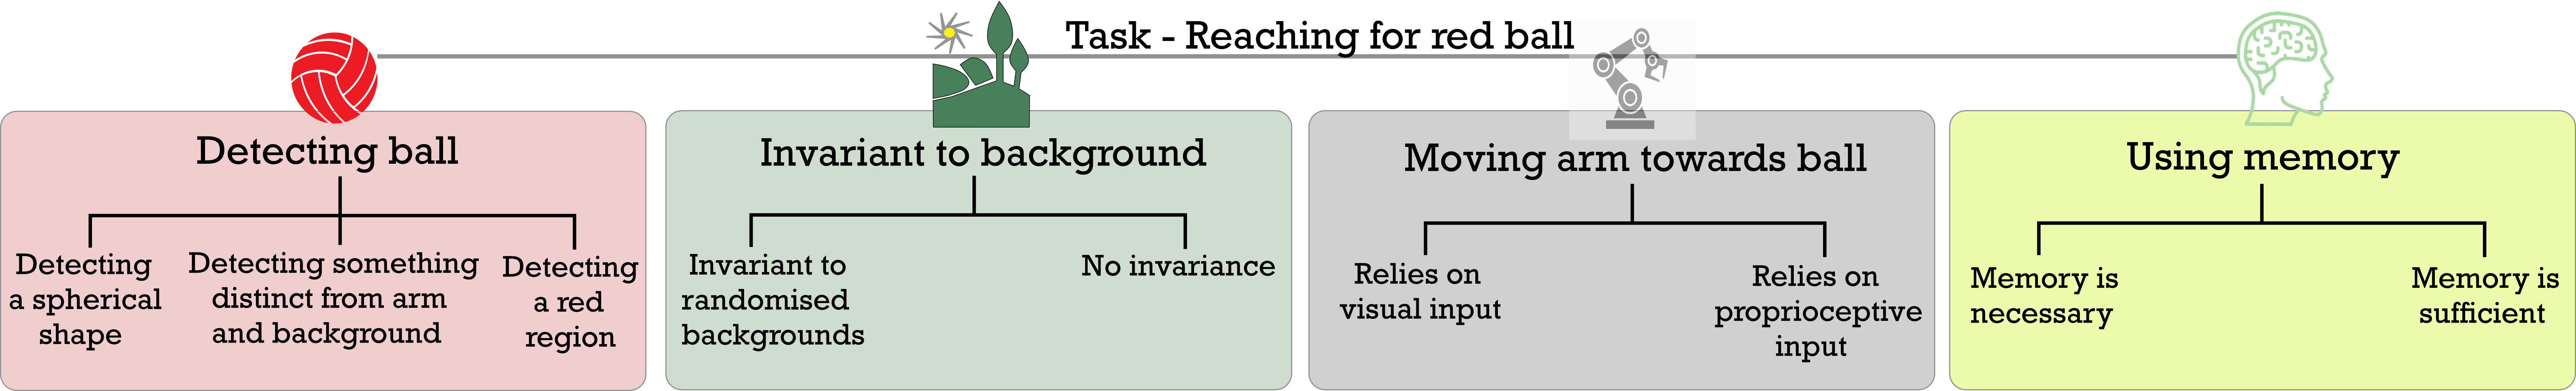
\includegraphics[width=\linewidth]{figures/chapter6/strategies.png}
  \caption{The range of strategies an agent may learn to use when trained to reach a red target, which we split into three components. Firstly, the agent must visually localise the target---which can be accomplished by detecting red, spherical objects, or simply anything with a significant red component. Secondly, the agent can use vision and/or proprioception to guide its arm to the target. Finally, the agent may accomplish the task with varying levels of robustness to changes in the rest of the visual scene. Using a range of analyses, we show that agents trained to accomplish the same task learn different subsets of these strategies, depending on their training conditions.}
  \label{fig:strategies}
\end{figure*}

Specifically, we train different robots with vision-based inputs to perform the task of reaching for a (red) target, and then use different techniques (Subsection \ref{sec:nn_interpretability}) to understand what features of the environment the policies react to. Under certain training settings, the agent may localise the target by simply looking for anything red, and it is only under more challenging training conditions that the agent utilises both colour and shape. Clearly, the latter strategy better represents what we want the agent to learn, while the former is merely a ``shortcut'' \cite{geirhos2020shortcut}.

\hypertarget{training-conditions}{%
\subsection{Training Conditions}\label{training-conditions}}
We vary training conditions over 3 different axes: 2 different robots with different morphologies and control schemes, using vision-only vs.~vision + proprioception, and training with/without visual \emph{domain randomisation} (DR). This results in 8 different configurations (Figure \ref{fig:axes}), which we found sufficient to uncover a large compositional space of strategies (Figure
\ref{fig:strategies}).

\begin{figure}
  \centering
  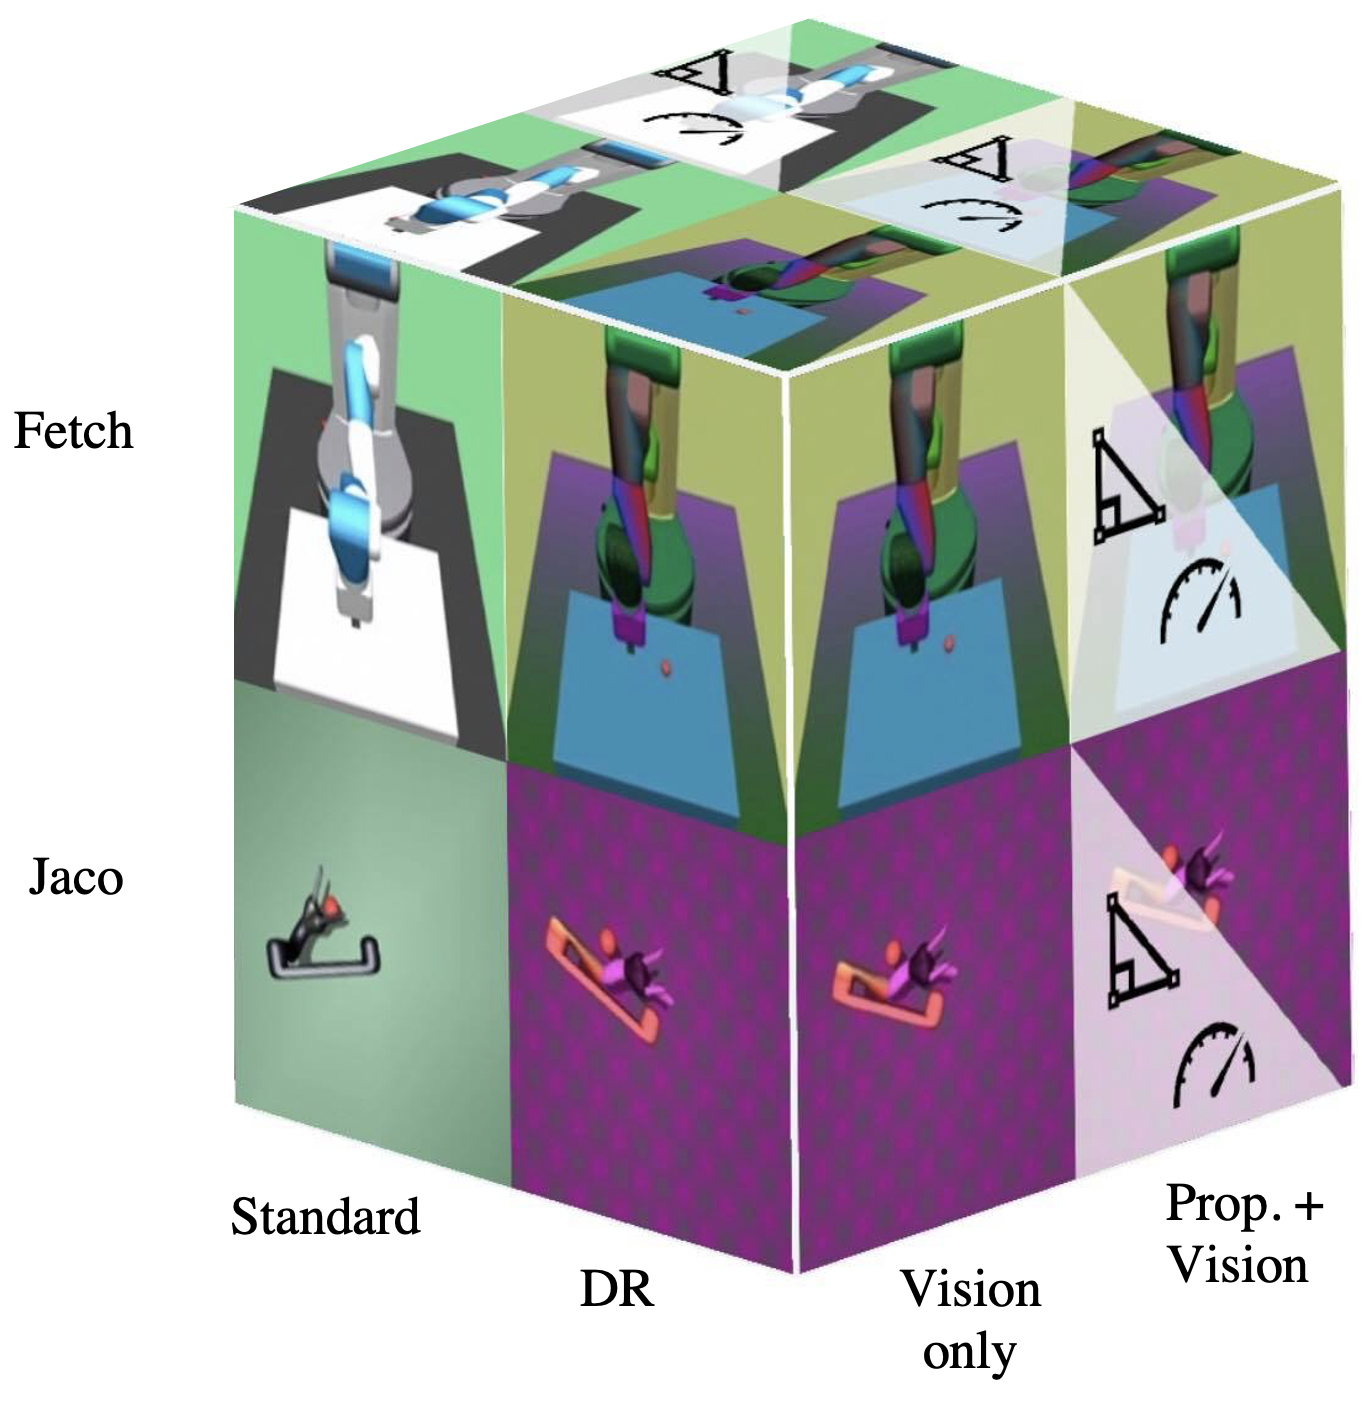
\includegraphics[width=0.85\linewidth]{figures/chapter6/axes.png}
  \caption{The 8 different experimental conditions: 2 robots (Fetch vs. Jaco), 2 input modalities (vision vs. vision + proprioception), 2 visual conditions (DR vs. no DR).}
  \label{fig:axes}
\end{figure}

We chose these 3 axes for the purpose of studying \emph{representation learning} in robotics tasks. The difference in the design of the robots, as well as a 2D vs.~3D target space (Subsection \ref{sec:environments}), results in one task being more difficult---in terms of both inferring the position of the target, as well as in the control. While task complexity is not a transitive property, the representations learned do reflect the difference between these tasks: for instance, localisation of the target in the latter case requires more complex image processing (Subsection \ref{sec:activation_maximisation}).

For real-world deployment, one would want to use as many sensors as it is feasible to use. However, we are interested in how the absence of certain input modalities can affect learning, as this changes how the agent is able to extract information from the environment. While one might expect robots equipped with proprioceptive sensors to use these alone for pose estimation, agents can also learn to utilise vision if extracting pose from images is simple (Subsection \ref{sec:saliency_maps}).

\begin{figure}
  \centering
  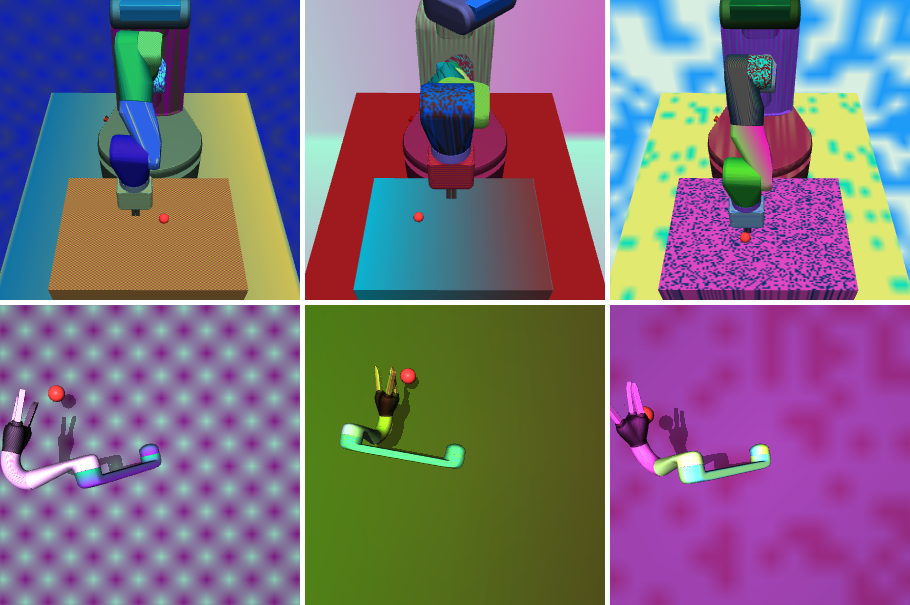
\includegraphics[width=\linewidth]{figures/chapter6/domain_random.png}
  \caption{Examples of visual domain randomisation in our Fetch (top) and Jaco (bottom) robotics experiments.}
  \label{fig:dr_example}
\end{figure}
\setlength{\textfloatsep}{5pt}

Finally, analogously to how \emph{data augmentation}~\cite{lecun1998gradient,shorten2019survey} can be used to improve the generalisation of models in supervised learning settings, \emph{domain randomisation} (Figure \ref{fig:dr_example}) is a common training paradigm in ``sim2real'' approaches for learning real-world robotics control~\cite{andrychowicz2018learning,james2017transferring,peng2018sim,sadeghi2017cad2rl,tobin2017domain}. In DR, various properties of the simulation are varied, altering anything from the positions or dynamical properties of objects to their visual appearance, resulting in an expansion of the training domain. We therefore test how the agents trained with or without DR differ. Supporting previous results, we show that agents trained with DR are more robust to out-of-distribution (OoD) perturbations (Subsection \ref{sec:test_scenarios}). In our experiments, we use a standard visual DR setup, which is described in Table \ref{tbl:random_summary} and visualised in Figure \ref{fig:random_vis}.

\begin{figure}
  \centering
  \begin{subfigure}{0.32\columnwidth}
    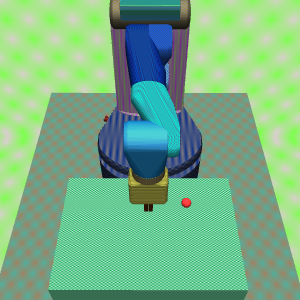
\includegraphics[width=\linewidth]{figures/chapter6/rand_checker.png}
    \subcaption{checkerboard}
  \end{subfigure}
  \begin{subfigure}{0.32\columnwidth}
    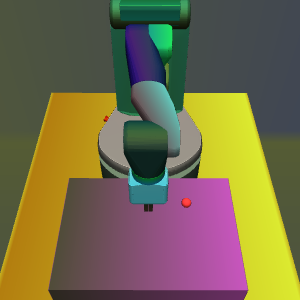
\includegraphics[width=\linewidth]{figures/chapter6/rand_gradient.png}
    \subcaption{gradient}
  \end{subfigure}

  \begin{subfigure}{0.32\columnwidth}
    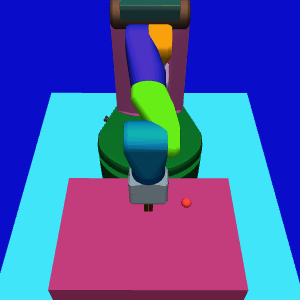
\includegraphics[width=\linewidth]{figures/chapter6/rand_rgb.png}
    \subcaption{flat\_rgb}
  \end{subfigure}
  \begin{subfigure}{0.32\columnwidth}
    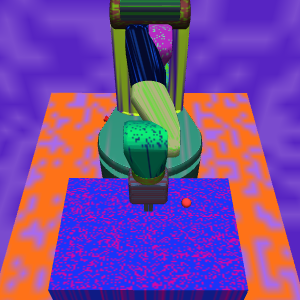
\includegraphics[width=\linewidth]{figures/chapter6/rand_noise.png}
    \subcaption{noise}
  \end{subfigure}
  \caption{Visualisation of different DR textures used during training: (a) checkerboard, (b) gradient, (c) flat\_rgb, (d) noise.}
  \label{fig:random_vis}
\end{figure}

DRL agents trained in standard simulators (due to the sample inefficiency of DRL algorithms) do not directly transfer to the real world. However, agents trained in simulators with DR can, which makes them of particular interest to study. It is common knowledge that while training in simulation is simpler, differences between the simulated and real worlds introduces a \emph{reality gap}~\cite{jakobi1995noise}. Of the several ways to address this gap---including fine-tuning a DRL agent on the real world~\cite{rusu2017sim}, performing system identification to reduce the domain gap~\cite{chebotar2018closing}, or explicitly performing domain adaptation~\cite{tzeng2015towards}---DR is unique in that it is essentially a form of data augmentation that only affects the input data, without changing the initial model or training objective. Thus, by comparing agents trained with DR against agents trained without, we expect to uncover what \emph{strategies} they learn that would allow generalisation in the real world (as opposed to, adaptation to the real world). For example, some of the robustness of our DR agents comes through learning to perform some form of state estimation implicitly (Subsection \ref{sec:recurrent_ablation}).

\begin{table}
  \label{tbl:random_summary}
  \centering
  \resizebox{\linewidth}{!}{
  \begin{tabular}{c|c|c}
    \toprule
    No. & Option & Description \\
    \midrule
   1 & checkerboard & Render checkerboard pattern with two random RGB colours\\
   2 & gradient & Render gradient in vertical/horizontal direction with two random RGB colours\\
   3 & flat\_rgb & Render single random RGB colour\\
   4 & noise & Render artificial noise with two random RGB colours\\
    \bottomrule
  \end{tabular}}
   \caption{DR textures used during training. At every environment timestep, for each component (e.g., robotic arm, skybox, table; the Jaco robot has 13 components, and the Fetch robot has 19 components), the appearance of the component is rendered using a sequential sampling process. In the first step of the sampling process, one of each of the 4 possible choices is made with the same probability, then the subsequent appearance of each component is determined by a second draw, described in the rightmost column of the table. Each RGB channel is drawn uniformly from $\{0 \ldots 255\}$. The details of each option are described in Table~\ref{tbl:texture_expression}.}
\end{table}

\begin{table}
  \label{tbl:texture_expression}
  \centering
  \resizebox{\linewidth}{!}{
  \begin{tabular}{c|c|c}
    \toprule
    No. & Option & Expression \\
    \midrule
   1 & checkerboard & texture\_mat[x, y] = rgb1 \textbf{if} (x + y) $\%$ 2 == 0 \textbf{else} rgb2\\
   2 & gradient & texture\_mat[x, y] = (1 - p) $\cdot$ rgb1 + p $\cdot$ rgb2, vertical: p = y / (height - 1), horizontal: p = x / (width - 1)\\
   3 & flat\_rgb & texture\_mat[x, y] = rgb1\\
   4 & noise & texture\_mat[x, y] = rgb1 \textbf{if} p > 0.9 \textbf{else} rgb2, p $\sim$ U(0, 1)\\
    \bottomrule
  \end{tabular}
  }
\caption{Python pseudocode describing the DR texture generators. rgb1 and rgb2 are random RGB colours; the value of each RGB channel is drawn uniformly from $\{0 \ldots 255\}$.}
\end{table}

\hypertarget{generalisation}{%
\subsection{Generalisation}\label{generalisation}}

The study of how DRL agents generalise has received considerable
interest in the DRL community recently
\cite{cobbe2018quantifying, justesen2018procedural, packer2018assessing, witty2018measuring, zhang2018dissection, zhao2019investigating}. As RL agents are typically trained and evaluated on the same environment, generalisation requires changes to the traditional paradigm. In particular, works in this area have also focused on procedural content generation and OoD tests to evaluate generalisation. In this paper, we not only quantitatively evaluate generalisation, but also use a wide suite of interpretability methods to try and understand why our trained agents act the way they do. Furthermore, we are the first to perform an in-depth study focused on DR. One of our findings is that, depending on the training conditions, we can observe a failure of agents trained with DR to generalise to the much simpler default visuals of the simulator (Subsection \ref{sec:domain_shift}), highlighting that conditions other than DR can have a significant effect on generalisation.

\hypertarget{interpretability}{%
\subsection{Interpretability}\label{interpretability}}

While our OoD tests (Subsection \ref{sec:test_scenarios}) provide a quantitative measure by which we can probe the performance of trained agents under various conditions, they treat the trained agents as black boxes. However, with full access to the internals of the trained models and even control over the training process, we can delve even further into the models. Using common interpretability tools such as saliency maps~\cite{morch1995visualization, selvaraju2017grad, sundararajan2017axiomatic, zeiler2014visualizing}
and dimensionality reduction methods
~\cite{maaten2008visualizing, mcinnes2018umap, pearson1901liii} for
visualising NN activations~\cite{rauber2017visualizing}, we can obtain
information on why agents act the way they do. The results of these
methods work in tandem with our OoD tests, as matching performance to
the qualitative results allows us to have greater confidence in
interpreting the latter; in fact, this process allowed us to debug and
improve upon an existing saliency map method, as detailed in Subsection
\ref{sec:back_saliency_maps}.
{Similarly to prior work}\footnote{Based on interpreting
  standard DRL agents, as opposed to constructing more interpretable
  agents.} on interpretability in DRL agents~\cite{atrey2020exploratory, greydanus2018visualizing, jaunet2020drlviz, meyes2020you, olson2021counterfactual, puri2020explain, rupprecht2020finding, such2018atari, zahavy2016graying}
{we use common methods: saliency maps (Subsection \ref{sec:back_saliency_maps}), activation maximisation (Subsection \ref{sec:act_max}), unit ablations (Subsection \ref{sec:unit_abl}) and dimensionality reduction (Subsection \ref{sec:act_an}).}
In addition, we use layer re-initialisation (Subsection
\ref{sec:layer_abl}), recurrent ablations (Subsection
\ref{sec:recurrent_abl}), entanglement (Subsection \ref{sec:act_an}),
and a novel quantitative measure for spatial structure in convolutional
filters (Subsection \ref{sec:spectral}).


\hypertarget{summary-of-findings}{%
\subsection{Summary of Findings}\label{summary-of-findings}}

Under our set of experimental conditions, we show that our agents
trained with DR:

\begin{itemize}
\item require more representational learning capacity (Subsection \ref{sec:layer_ablations}),
\item are more robust to visual changes in the scene, exhibiting generalisation to unseen local/global perturbations (Subsection \ref{sec:test_scenarios}),
\item use a smaller set of more reliable visual cues when not provided proprioceptive inputs (Subsection \ref{sec:saliency_maps}),
\item more heavily rely on recurrent processing (Subsection \ref{sec:recurrent_ablation}),
\item have filters that have higher norms or greater spatial structure (Subsection \ref{sec:statistical_and_structural}), which respond to more complex spatial patterns (Subsection \ref{sec:activation_maximisation}),
\item learn more robust (Subsection \ref{sec:unit_ablations}) and \textit{entangled} \cite{frosst2019analyzing} representations (Subsection \ref{sec:activation_analysis}),
\item and can ``overfit'' to DR visuals (Subsection \ref{sec:domain_shift}).
\end{itemize}

Furthermore, we characterise what strategies (Figure
\ref{fig:strategies}) agents learn as a result of being trained under
different conditions. In our discussion (Section \ref{sec:discussion}),
we revisit what this entails for future work on sim2real methods, and
end with a set of recommendations for those interesting in applying
interpretability methods to DRL agents.

\hypertarget{overview}{%
\subsection{Overview}\label{overview}}

The rest of the paper is organised as the follows: In Section
\ref{sec:methods}, we introduce RL, and the neural network
interpretability techniques used in this work. In Section
\ref{sec:experiments}, we detail our simulated environments, DRL agent
network structure, training details, and test scenarios. In Section
\ref{sec:model_analysis}, we conduct an exhaustive analysis on the
trained models using a broad suite of interpretability techniques.
Finally, in Section \ref{sec:discussion}, we discuss our findings, and
provide recommendations for applying interpretability techniques to DRL
agents. The code used in this paper is available at:
\url{https://github.com/TianhongDai/domain-rand-interp}.
% method
\hypertarget{methods}{%
\section{Methods}\label{methods}}
\label{sec:methods}

\hypertarget{neural-network-interpretability}{%
\subsection{Neural Network
Interpretability}\label{neural-network-interpretability}}

\label{sec:nn_interpretability}

The recent success of machine learning (ML) methods has led to a renewed
interest in trying to interpret trained models. In this work, we are
primarily concerned with scientific understanding, but our
considerations are grounded in other properties necessary for eventual
real-world deployment, such as robustness to OoD inputs.

The challenge that we face is that, unlike other ML algorithms that are
considered interpretable by design (such as decision trees or nearest
neighbours \cite{freitas2014comprehensible}), standard NNs are
generally considered black boxes. However, given decades of research
into methods for interpreting NNs
\cite{craven1996extracting, morch1995visualization}, we now have a
range of techniques at our disposal \cite{guidotti2018survey}. Beyond
simply looking at test performance (a measure of interpretability in its
own right \cite{doshi2017towards}), we will focus on a variety of
techniques that will let us examine trained NNs both in the context of,
and independently of, task performance. In particular, we discuss
saliency maps (Subsection \ref{sec:back_saliency_maps}), activation
maximisation (Subsection \ref{sec:act_max}), weight visualisations
(Subsection \ref{sec:weight_vis}), statistical and structural weight
characterisations (Subsection \ref{sec:stat_struct_weight}), unit
ablations (Subsection \ref{sec:unit_abl}), layer re-initialisation
(Subsection \ref{sec:layer_abl}), recurrent ablations (Subsection
\ref{sec:recurrent_abl}) and activation analysis (Subsection
\ref{sec:act_an}). By utilising a range of techniques we hope to cover
various points along the trade-off between fidelity and interpretability
\cite{ribeiro2016should}.

\hypertarget{saliency-maps}{%
\subsubsection{Saliency Maps}\label{saliency-maps}}

\label{sec:back_saliency_maps}

Saliency maps are one of the most common techniques used for
understanding the decisions made by NNs, and in particular,
convolutional NNs (CNNs). In line with prior work on interpreting DRL
agents \cite{greydanus2018visualizing}, we use occlusion-based methods,
in which parts of the image are masked to perform a sensitivity analysis
with respect to the change in the network's outputs. The original method
introduced by Zeiler et al. \cite{zeiler2014visualizing} proposes
running a (grey, square) mask over the input and tracking how the
network's outputs change in response. Greydanus et al.
\cite{greydanus2018visualizing} applied this method to understanding
actor-critic-based DRL agents, using the resulting saliency maps to
examine strong and overfitting policies; they however noted that a grey
square may be perceived as part of a grey object, and instead used a
localised Gaussian blur to add ``spatial uncertainty''. The saliency
value \(S_{m,n}\) for each input location \((m, n)\) is the Euclidean
distance between the original output and the output given the input
\(\mathbf{x}_{m, n}^{occ}\) which has been occluded at location
\((m, n)\): \begin{align}
S_{m, n} = \lVert F(\mathbf{x}) - F(\mathbf{x}_{m, n}^{occ}) \rVert_2,
\end{align} \noindent where \(\lVert\cdot\rVert_p\) denotes the
\(\ell_p\)-norm.

However, we found that certain trained agents sometimes confused the
blurred location with the target location---a failing of the attribution
method against noise/distractors \cite{kindermans2016investigating},
and not necessarily the model itself. {Atrey et al.}
\cite{atrey2020exploratory} {identified this issue of applying saliency methods to DRL agents as modifying observations in a manner that is incongruent with the true environment's state and generative process, and proposed intervening directly in the environment in order to employ counterfactual methods. However, in general this level of control over the environment is not possible.}
Motivated by the methods that compute interpretations against reference
inputs
\cite{bach2015pixel, ribeiro2016should, shrikumar2017learning, sundararajan2017axiomatic},
we replaced the Gaussian blur with a mask\footnote{Replacing a circular
  region of 5px radius around the \((m, n)\) location.} derived from a
baseline input, which roughly represents what the model would expect to
see on average. Intuitively, this acts as a counterfactual, revealing
what would happen if the specific part of the input was not there. For
this we averaged over frames collected from our standard evaluation
protocol (see Subsection \ref{sec:environments} for details), creating
an average input to be used as an improved mask for the occlusion-based
method (Figure \ref{fig:saliency_baseline}). Unless specified otherwise,
we use our average input baseline for all occlusion-based saliency maps.
Contemporaneous work has examined the use of more advanced baselines for
gradient-based saliency map methods \cite{sturmfels2020visualizing}. {Another recent work has introduced a more robust DRL-specific saliency method}
\cite{puri2020explain}{, but it is only applicable to agents which learn a state-action value function over discrete action spaces.}

\begin{figure}
  \centering
  \begin{subfigure}{0.32\columnwidth}
    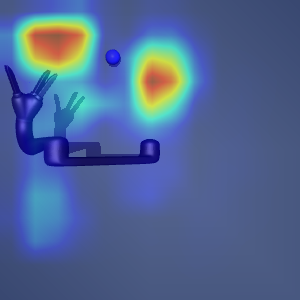
\includegraphics[width=\linewidth]{figures/chapter6/occ_jaco_baseline}
    \subcaption{Occ. (Gaussian)}
  \end{subfigure}
  \begin{subfigure}{0.32\columnwidth}
    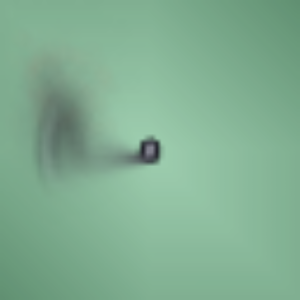
\includegraphics[width=\linewidth]{figures/chapter6/average_map_jaco_large.png}
    \subcaption{Avg. $\mathbf{x}^{base}$}
  \end{subfigure}

  \begin{subfigure}{0.32\columnwidth}
    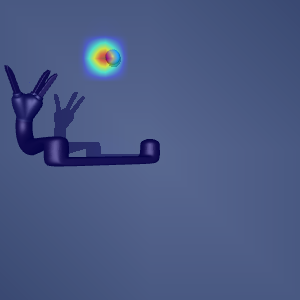
\includegraphics[width=\linewidth]{figures/chapter6/occ_jaco_average_map.png}
    \subcaption{Occ. (avg. $\mathbf{x}^{base}$)}
  \end{subfigure}
  \begin{subfigure}{0.32\columnwidth}
    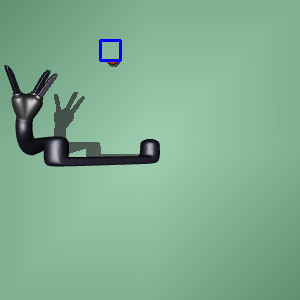
\includegraphics[width=\linewidth]{figures/chapter6/average_map_mask.png}
    \subcaption{Avg. $\mathbf{x}^{base}$ mask}
  \end{subfigure}
  \caption{Occlusion-based saliency map method (a) improved (c) by the use of an \textit{average image} (b, d). Occlusion (occ.) with the \textit{default Gaussian blur} (a) shows additional artifacts. By creating an average image (b) from a large set of trajectories, we can form an improved baseline for occlusion (c); the usage of the average image as the occlusion (with a blue outline added for emphasis) is pictured in (d).}
  \label{fig:saliency_baseline}
\end{figure}

\hypertarget{activation-maximisation}{%
\subsubsection{Activation Maximisation}\label{activation-maximisation}}

\label{sec:act_max}

Gradients can also be used to try and visualise what maximises the
activation of a given neuron/channel. This can be formulated as an
optimisation problem, using projected gradient ascent in the input space
(where after every gradient step the input is clamped back to within
\([0, 1]\)) \cite{erhan2009visualizing}. Although this would ideally
show what a neuron/channel is selective for, unconstrained optimisation
may end up in solutions far from the training manifold
\cite{mahendran2015understanding}, and so a variety of regularisation
techniques have been suggested for making qualitatively superior
visualisations. We experimented with some of ``weak regularisers''
\cite{olah2017feature}, and found that a combination of frequency
penalisation (Gaussian blur) \cite{nguyen2015deep} and transformation
robustness (random scaling and translation/jitter)
\cite{mordvintsev2015inceptionism} worked best, although they were not
sufficient to completely rid the resulting visualisations of the high
frequency patterns caused by strided convolutions
\cite{odena2016deconvolution}. We performed the optimisation procedure
for activation maximisation for 20 iterations, applying the
regularisation transformations and taking gradient steps in the
\(\ell_2\)-norm \cite{madry2018towards} with a step size of 0.1.
Pseudocode for our method, applied to a trained network \(f\), is
detailed in Algorithm \ref{alg:act_max}.

\begin{algorithm}
\caption{Activation maximisation procedure with transformation robustness, frequency penalisation and $\ell_2$-norm gradient updates.}
\label{alg:act_max}
\begin{algorithmic}
\STATE $f' \gets \text{network } f \text{ truncated at intermediate layer}$
\STATE $i \gets \text{optimisation iterations}$
\STATE $n \gets \text{neuron/channel index}$
\STATE $\alpha \gets \text{step size}$
\STATE $x \sim U(0, 1) \text{ with dimensionality } 3 \times \text{height} \times \text{width}$
\FOR{$i$ steps}
  \STATE $x \gets RandomScale(x)$
  \STATE $x \gets RandomJitter(x)$
  \STATE $x \gets GaussianBlur(x)$
  \STATE $\mathcal{L} \gets \text{mean}(f'(x)_n)$
  \STATE $x \gets x + \alpha\frac{\nabla\mathcal{L}_x}{\Vert \nabla\mathcal{L}_x \Vert_2}$
  \STATE $x \gets \min(\max(x, 0), 1)$
\ENDFOR
%\STATE 
\RETURN $x$
\end{algorithmic}
\end{algorithm}

\hypertarget{weight-visualisations}{%
\subsubsection{Weight Visualisations}\label{weight-visualisations}}

\label{sec:weight_vis}

It is possible to visualise both convolutional filters and
fully-connected weight matrices as images. Part of the initial
excitement around DL was the observation that CNNs trained on object
recognition would learn frequency-, orientation- and colour-selective
filters \cite{krizhevsky2012imagenet}, and more broadly might reflect
the hierarchical feature extraction within the visual cortex
\cite{yamins2016using}. However, as demonstrated by Such et al.
\cite{such2018atari}, DRL agents can perform well with spatially
unstructured filters, although they did find a positive correlation
between spatial structure and performance for RL agents trained with
gradients. Consistent with these findings, we find that spatial
structure is correlated with OoD performance (Subsection
\ref{sec:test_scenarios}). To support this, we developed a novel
quantitative measure to compare filters, which we discuss below.

\hypertarget{statistical-and-structural-weight-characterisations}{%
\subsubsection{Statistical and Structural Weight
Characterisations}\label{statistical-and-structural-weight-characterisations}}

\label{sec:stat_struct_weight}

\hypertarget{magnitude}{%
\paragraph{Magnitude}\label{magnitude}}

\label{sec:magnitude}

A traditional measure for the ``importance'' of individual neurons in a
weight matrix is their magnitude, as exemplified by utilising weight
decay as a regulariser \cite{hanson1989comparing}. Similarly,
convolutional filters, considered as one unit, can be characterised by
their \(\ell_1\)-norms. Given that NN weights are typically randomly
initialised with small but non-zero values
\cite{glorot2010understanding, lecun1998efficient}, the presence of
many zeros or large values indicate significant changes during training.
We can compare these both across trained agents, and across the training
process (although change in magnitude may not correspond with a change
in task performance \cite{zhang2019all}).

\hypertarget{spectral-analysis}{%
\paragraph{Spectral Analysis}\label{spectral-analysis}}

\label{sec:spectral}

Convolutional filters are typically initialised pseudo-randomly, so that
there exists little or no spatial correlation within a single unit. We
hence propose using the 2D discrete power spectral density (PSD) as a
way of assessing the spatial organisation of convolutional filters, and
the power spectral entropy (PSE) as a measure of their complexity. Given
the mean-centred\footnote{Offsetting the mean exposes the
  \emph{relative} spatial structure.} 2D spatial-domain filter,
\(\mathbf{W}_{m, n}\), its corresponding spectral representation,
\(\mathbf{\hat{W}}_{u, v}\), can be calculated via the 2D discrete
Fourier transform of the original filter pattern (\(j=\sqrt{-1}\)):
\begin{align}
\mathbf{\hat{W}}_{u, v} = \sum_{m=0}^{M-1}\sum_{n=0}^{N-1}W_{m, n} \exp \left [ -\frac{j 2\pi}{MN}(u m + v n) \right ],
\end{align} \noindent and its PSD, \(\mathbf{S}_{u, v}\), from the
normalised squared amplitude of the spectrum: \begin{align}
\mathbf{S}_{u, v} = \frac{1}{U V} \left|\mathbf{\hat{W}}_{u, v}\right|^2,
\end{align} \noindent where \((m, n)\) are spatial indices, \((u, v)\)
are frequency indices, \((M, N)\) is the spatial extent of the filter,
and \((U, V)\) is the frequency extent of the filter.

When renormalised such that the sum of the PSD is 1, the PSD may be
thought of as a probability mass function over a dictionary of
components from a spatial Fourier transform. We can treat each location
\((u, v)\) in Fourier space as a symbol, and its corresponding value at
\(\mathbf{S}_{u, v}\) as the probability of that symbol appearing. The
PSE is then simply the Shannon entropy of this distribution, which we
use as a measure of spatial (dis)organisation. In our analysis
(Subsection \ref{sec:statistical_and_structural}), we include statistics
calculated over randomly initialised networks as a baseline. As the
initial weights for units are typically drawn independently from a
normal or uniform distribution, this leads to a fairly flat PSD with PSE
close to \(\log(MN)\)---an upper-bound on PSE.

One weakness of spectral analysis is that these measures will fail to
pick up strongly localised spatial features, as such filters would also
result in a roughly uniform PSD. In practice, global structure is still
useful to quantify, and matches well with human intuition (Figure
\ref{fig:entropy_vis}).

\begin{figure}
  \centering
  \begin{subfigure}{0.3\columnwidth}
    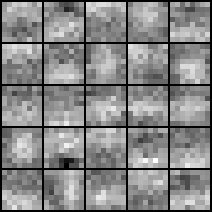
\includegraphics[width=\linewidth]{figures/chapter6/entropy_filter/bot_filts_dr}
    \subcaption{PSE = 2.63}
  \end{subfigure}
  \begin{subfigure}{0.3\columnwidth}
    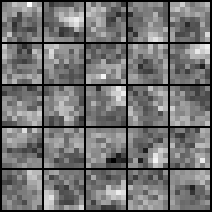
\includegraphics[width=\linewidth]{figures/chapter6/entropy_filter/mid_filts_dr}
    \subcaption{PSE = 3.19}
  \end{subfigure}
  \begin{subfigure}{0.3\columnwidth}
    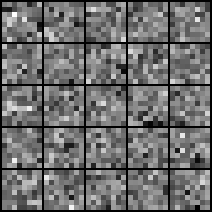
\includegraphics[width=\linewidth]{figures/chapter6/entropy_filter/top_filts_dr}
    \subcaption{PSE = 3.86}
  \end{subfigure}
  \caption{Convolutional filters from models trained with DR, with varying power spectral entropies, ranked from the lowest (a) to highest (c). The PSE value refers to the centre filter.}
  \label{fig:entropy_vis}
\end{figure}

Entropy as an information-theoretic measure has been used in DL in many
functions, from predicting neural network ensemble performance
\cite{hansen1990neural} to usage as a regulariser
\cite{khabou1999entropy} or pruning criteria \cite{luo2017entropy}
when applied to activations. Spectral entropy has been used as an input
feature for NNs
\cite{krkic1996eeg, misra2004spectral, srinivasan2005artificial, zheng1996digital},
but, to the best of our knowledge, not for quantifying aspects of the
network itself.

\hypertarget{unit-ablations}{%
\subsubsection{Unit Ablations}\label{unit-ablations}}

\label{sec:unit_abl}

Another way to characterise the importance of a single
neuron/convolutional filter is to remove it and observe how this affects
the performance of the NN: a large drop indicates that a particular unit
is by itself very important to the task at hand. More generally, rather
than only looking at performance, one might look for a large change in
the output. {While more sophisticated unit ablations have been applied in DRL}
\cite{meyes2020you}, {this has only been in the context of a control task with a low-dimensional symbolic state space}.

\hypertarget{layer-re-initialisation}{%
\subsubsection{Layer Re-initialisation}\label{layer-re-initialisation}}

\label{sec:layer_abl}

One can extend the concept of ablations to entire layers, and use this
to study the \emph{re-initialisation robustness} of trained networks
\cite{zhang2019all}. Typical neural network architectures, as used in
our work, are compositions of multiple parameterised layers, with
parameters \(\{\theta_1, \theta_2, \ldots, \theta_L\}\), where \(L\) is
the depth of the network. Using \(\theta_l^t\) to denote the set of
parameters of layer \(l \in [1, L]\) at training epoch \(t \in [1, T]\)
over a maximum of \(T\) epochs, we can study the evolution of each
layer's parameters over time---for example through the change in the
\(\ell_\infty\)- or \(\ell_2\)-norm of the set of parameters.

Zhang et al. \cite{zhang2019all} proposed re-initialisation robustness
as a measure of how important a layer's parameters are with respect to
task performance over the span of the optimisation procedure. After
training, for a given layer \(l\), re-initialisation robustness is
measured by replacing the parameters \(\theta_l^T\) with parameters
checkpointed from a previous timepoint \(t\), that is, setting
\(\theta_l^T \leftarrow \theta_l^t\), and then re-measuring task
performance. They observed that for common CNN architectures trained for
object classification, while the parameters of the latter layers of the
networks tended to change a lot by the \(\ell_\infty\)- and
\(\ell_2\)-norms, the same layers were robust to re-initialisation at
checkpoints early during the optimisation procedure, and even to the
initialisation at \(t = 0\). In the latter case, the parameters are
independent of the training data, which means that the effective number
of parameters is lower than the total number of parameters. Given that
the effective number of parameters is a better measure for model
complexity than total number, this potentially allows us to
differentiate between models with the same architecture. Unlike Zhang et
al. \cite{zhang2019all}, we use re-initialisation robustness to study
the effect of task complexity (training with and without DR, and with
and without proprioceptive inputs), but with networks of similar
capacity.

\hypertarget{recurrent-ablation}{%
\subsubsection{Recurrent Ablation}\label{recurrent-ablation}}

\label{sec:recurrent_abl}

When using recurrent units in the network architecture, we can test if
non-trivial recurrent dynamics are being used by forcing the hidden
state to be constant. If the performance of the agent degrades, then it
is somehow using the recurrent dynamics to perform the task---although
it is difficult to say what the exact ``strategy'' might be. However, if
the performance drop is zero or minimal, then the recurrency is not
being utilised. The constant values of the hidden states should be set
to the empirical average of the values during normal operation, as
naively setting all values to zero could cause a considerable shift in
the distribution of expected inputs---as the hypothesis is that the
network may have learned a constant offset, rather than completely
ignoring the hidden state. {While it is possible to investigate the hidden states of DRL agents over time, visualising and inspecting a high-dimensional time series can be difficult, even for domain experts}
\cite{jaunet2020drlviz}.

\hypertarget{entanglement}{%
\subsubsection{Entanglement}\label{entanglement}}

\label{sec:act_an}

Finally, we consider analysing the internal activations of trained
networks. One of the primary methods for examining activations is to
take the high-dimensional vectors and project them to a
lower-dimensional space (commonly \(\mathbb{R}^2\) for visualisation
purposes) using dimensionality reduction methods that try and preserve
the structure of the original data \cite{rauber2017visualizing}. Common
choices for visualising activations include both principal components
analysis (PCA; a linear projection)
\cite{elman1989representation, pearson1901liii} and t-distributed
stochastic neighbor embedding (t-SNE; a nonlinear projection)
\cite{hamel2010learning, maaten2008visualizing, mnih2015human}. {Prior work has used t-SNE to explore the state visitations of DRL agents, clustering states which are associated with similar actions}
\cite{mnih2015human, zahavy2016graying}.

While these works qualitatively examine the projections of the
activations for a single network, or compare them across trained
networks, we additionally introduce a method to use the projections
quantitatively. In supervised learning settings, one can examine class
overlap in the projected space \cite{rauber2017visualizing}. In our RL
setting there is no native concept of a ``class'', but we can instead
use activations taken under different OoD test scenarios (Subsection
\ref{sec:test_scenarios}) to see (beyond the generalisation performance)
how the internal representations of the trained networks vary under the
different scenarios. Specifically, we measure \emph{entanglement} (``how
close pairs of representations from the same class are, relative to
pairs of representations from different classes''
\cite{frosst2019analyzing}) using the soft nearest neighbour loss,
\(\mathcal{L}_{SNN}\) \cite{salakhutdinov2007learning}, defined over a
batch of size \(B\) with samples \(\mathbf{x}\) and classes \(y\) (where
in our case \(\mathbf{x}\) is a projected activation and \(y\) is a test
scenario) with temperature \(T\) (and using \(\delta_{i,j}\) as the
Kronecker-delta):

\begin{eqnarray}
\mathcal{L}_{SNN} = \frac{1}{B} \sum_{n=1}^B \left ( \log \left [ \sum_{b=1}^B (1-\delta_{b,n}) \cdot e^{-\frac{\lVert \mathbf{x}_n - \mathbf{x}_b \rVert_2^2}{T}} \right ] \right . \nonumber \\
\left . -\log \left [\sum_{a=1}^B (1-\delta_{a,n}) \cdot \delta_{y_a,y_n} \cdot e^{-\frac{\lVert \mathbf{x}_n - \mathbf{x}_a \rVert_2^2}{T}} \right ] \right )
\end{eqnarray}

In particular, if representations between different test scenarios are
highly entangled, this indicates that the network is largely invariant
to the factors of variation between the different scenarios. Considering
DR as a form of data augmentation, this is what we might expect of
networks trained with DR.

\hypertarget{experiments}{%
\section{Experiments}\label{experiments}}

\label{sec:experiments}

\hypertarget{environments}{%
\subsection{Environments}\label{environments}}

\label{sec:environments}

We base our experiments on the common setup of performing
target-reaching with visuomotor control. The tasks involve moving the
end effector of a robot arm to reach a randomly positioned target during
each episode, with visual (one RGB camera view) and sometimes
proprioceptive (joint positions, angles and velocities) input provided
to the agent. Unlike many DRL experiments where the position of the
joints and the target are explicitly provided \cite{plappert2018multi},
in our setup the agent must infer the position of the target, and
sometimes itself, purely through vision. Importantly, we use two robotic
arms---the Fetch Mobile Manipulator and the KINOVA JACO Assistive
robotic arm (pictured in Figure \ref{fig:robot_setups}; henceforth
referred to as Fetch and Jaco, respectively)---which have different
control schemes and different visual appearances. This leads to changes
in the relative importance of the visual and proprioceptive inputs,
which we explore in several of our experiments. These robot environments
are commonly used within the DRL literature
\cite{andrychowicz2017hindsight, gu2017deep, rusu2017sim} and,
therefore, adopting these in our experiments enables both comparison to
prior work and applicability to the DRL field.

\begin{figure}
  \centering
  \begin{subfigure}{0.49\columnwidth}
    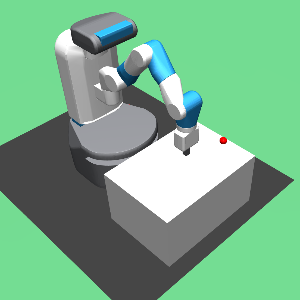
\includegraphics[width=\linewidth]{figures/chapter6/fetch_sim.png}
    \subcaption{Fetch enviroment}
  \end{subfigure}
  \begin{subfigure}{0.49\columnwidth}
    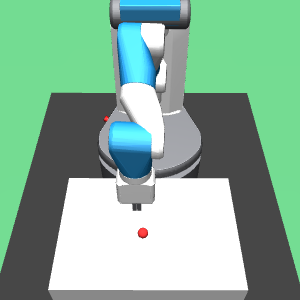
\includegraphics[width=\linewidth]{figures/chapter6/fetch_view.png}
    \subcaption{Fetch camera view}
  \end{subfigure}
  \\
  \begin{subfigure}{0.49\columnwidth}
    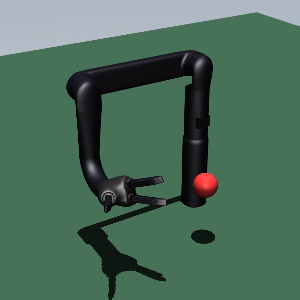
\includegraphics[width=\linewidth]{figures/chapter6/jaco_sim.png}
    \subcaption{Jaco environment}
  \end{subfigure}
%  \begin{subfigure}{0.32\columnwidth}
%    \includegraphics[width=\linewidth]{jaco_side}
%    \subcaption{Jaco side view}
%  \end{subfigure}
  \begin{subfigure}{0.49\columnwidth}
    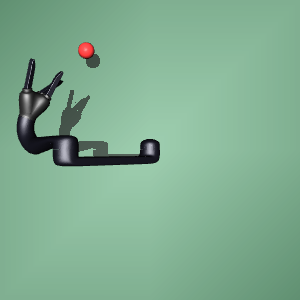
\includegraphics[width=\linewidth]{figures/chapter6/jaco_top.png}
    \subcaption{Jaco camera view}
  \end{subfigure}
  \caption{Fetch (a) and Jaco (c) environments, with associated camera views (b, d) that are provided as input to the agents.}
  \label{fig:robot_setups}
\end{figure}

The Fetch has a 7 degrees-of-freedom (DoF) arm, not including the
two-finger gripper. The original model and reaching task setup were
modified from the \texttt{FetchReach} task in OpenAI Gym
\cite{brockman2016openai, plappert2018multi} in order to provide an
additional camera feed for the agent (while also removing the
coordinates of the target from the input). The target can appear
anywhere on the 2D table surface. The agent has 3 sets of actions,
corresponding to position control of the end effector ({[}-5, 5{]} cm in
the x, y and z directions; gripper control is disabled).

The Jaco has been configured to be 6 DoF, with the 3 fingers disabled.
The target can appear anywhere within a 3D area to one side of the
robot's base. The agent has 6 sets of actions, corresponding to velocity
control of the arm joints ({[}-0.6, +0.6{]} rad/s). Due to the
difference in control schemes, 2D versus 3D target locations, and
homogeneous appearance of the Jaco, reaching tasks with the Jaco are
more challenging---particularly when proprioceptive input is not
provided to the agent. A summary of the different settings for the Fetch
and Jaco environments is provided in Table \ref{tbl:exp_setup}.

\begin{table}
  \caption{Summary of Fetch and Jaco experimental setups.}
  \label{tbl:exp_setup}
  \centering
  \begin{tabular}{c|cc}
    \toprule
    Setting & Fetch & Jaco \\
    \midrule
    Active (Total) DoF & 7 (8) & 6 (9) \\
    Target Range & $21 \times 31 \text{cm}^2$ & $40 \times 40 \times 40 \text{cm}^3$ \\
    Num. Test Targets & 80 & 250 \\
    Vision Input & $3 \times 64 \times 64$ & $3 \times 64 \times 64$ \\
    Proprioceptive Inputs & 30 & 18 \\
    Control Type & Position & Velocity \\
    Num. Actions & 3 & 6 \\
    Action Discretisation & 5 & 5 \\
    Control Frequency & 6.67Hz & 6.67Hz \\
    \bottomrule
  \end{tabular}
\end{table}

During training, target positions are sampled uniformly from within the
set range, with episodes terminating once the target is reached (within
10 cm of the target centre), or otherwise timing out in 100 timesteps.
The reward is sparse, with the only nonzero reward being +1 when the
target is reached. During testing, a fixed set of target positions,
covering a uniform grid over all possible target positions, are used; 80
positions in a 2D grid are used for Fetch, and 250 positions in a 3D
grid are used for Jaco. By using a deterministic policy and averaging
performance over the entire set of test target positions, we obtain an
empirical estimate of the probability of task success. Test episodes are
set to time out within 20 timesteps in order to minimise false positives
from the policy accidentally reaching the target.

We only randomise initial positions (for all agents) and visuals (for
some agents), but not dynamics, as this is still a sufficiently rich
task setup to explore. Henceforth we refer to agents trained with visual
randomisations as being under the DR condition, whereas agents trained
without are the standard (baseline) condition. Apart from the target, we
randomise the visuals of all other objects in the environment: the
robots, the table, the floor and the skybox. At the start of every
episode and at each timestep, we randomly alter the RGB colours,
textures and colour gradients of all surfaces (Figure
\ref{fig:dr_example}).

Importantly, there are several aspects that are not altered, as we also
want to test extrapolation to OoD scenarios (Subsection
\ref{sec:test_scenarios}). For example, one of the tests that we apply
to probe generalisation is to change a previously static
property---surface reflectivity, which is completely disabled during
training---and see how this affects the trained agents. All environments
were constructed in MuJoCo \cite{todorov2012mujoco}, a fast and
accurate physics simulator that is commonly used for DRL experiments.

\hypertarget{networks-and-training}{%
\subsection{Networks and Training}\label{networks-and-training}}

\label{sec:networks_training}

\begin{figure*}
  \centering
  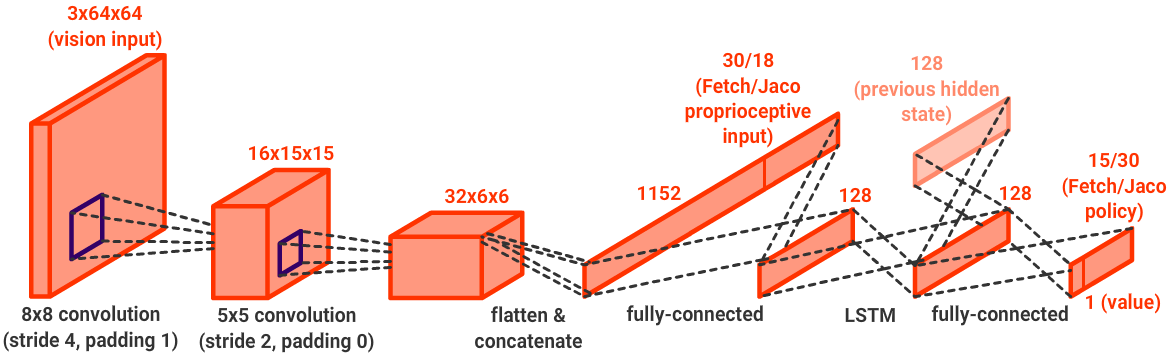
\includegraphics[width=0.85\linewidth]{figures/chapter6/network.png}
  \caption{Actor-critic network architecture.}
  \label{fig:network}
\end{figure*}

We utilise the same basic actor-critic network architecture for each
experiment, based on the recurrent architecture used by Rusu et al.
\cite{rusu2017sim} for their Jaco experiments. The architecture has 2
convolutional layers, a fully-connected layer, a long short-term memory
(LSTM) layer \cite{gers2000learning, hochreiter1997long}, and a final
fully-connected layer for the policy and value outputs; rectified linear
units were used at the output of the convolutional layers and first
fully-connected layer. Proprioceptive inputs, when provided, were
concatenated with the outputs of the convolutional layers before being
input into the first fully-connected-layer. The policy,
\(\pi(\cdot; \theta)\), is a product of independent categorical
distributions, with one distribution per action dimension. Weights were
initialised using orthogonal weight initialisation
\cite{ilyas2018deep, saxe2014exact} and biases were set to zero. The
specifics of the architecture are detailed in Figure \ref{fig:network}.

During training, a stochastic policy
\(\mathbf{a} \sim \pi(\mathbf{a}|\mathbf{s}; \theta)\) is used and
trained with PPO with clip ratio \(\epsilon = 0.1\), GAE trace decay
\(\lambda = 0.95\) and discount \(\gamma = 0.99\). Each epoch of
training consists of 32 worker processes collecting 128 timesteps worth
of data each, then 4 PPO updates with a minibatch size of 1024. We train
for up to \(5 \times 10^3\) epochs, using the Adam optimiser
\cite{kingma2014adam} with learning rate \(= 2.5 \times 10^{-4}\),
\(\beta\)s \(= \{0.9, 0.999\}\), and \(\epsilon = 1 \times 10^{-5}\).
\(\mathcal{L}_{value}\) is weighted by 0.5 and \(\mathcal{L}_{entropy}\)
is weighted by 0.01. If the max \(\ell_2\)-norm of the gradients exceeds
0.5 they are rescaled to have a max \(\ell_2\)-norm of 0.5
\cite{pascanu2013difficulty}. During testing, the deterministic policy
\(\mathbf{a} = \argmax_\mathbf{a} \pi(\mathbf{a}|\mathbf{s}; \theta)\)
is used. Our training was implemented using PyTorch
\cite{paszke2019pytorch}. Training each model (each random seed) for
the full number of timesteps takes 1 day on a GTX 1080Ti; we trained
models with 5 different seeds for each of the 8 conditions. The overall
setup is detailed in Algorithm \ref{alg:overall_algo}.

\begin{algorithm}
\caption{PPO + DR training.}
\label{alg:overall_algo}
\begin{algorithmic}
\REQUIRE environment $E$, actor network $\pi(a|s;\theta)$, critic network $V_{\pi}(s;\theta)$, number of training epochs $N$, number of timesteps to collect data $T$, number of PPO updates $M$, on-policy transition memory $\mathcal{B}$
\FOR{epoch $= 1, 2, \ldots, N$}
  \STATE $\mathcal{B} \gets \varnothing$
  \FOR{$t = 1, 2, \ldots, T$}
    \IF{$E$ has terminated}
      \STATE Reset $E$ and receive DR \indent\indent state $s_0$
    \ENDIF
    \STATE Sample an action $a_t \sim \pi(a|s_t;\theta)$
    \STATE Execute $a_{t}$ in $E$ and receive reward $r_t$, DR next \indent\indent state $s_{t+1}$, and $terminal$
    \STATE Store the transition $\left(s_t, a_t, r_t, s_{t+1}, terminal \right)$ in $\mathcal{B}$
  \ENDFOR
  \FOR{PPO update $= 1, 2, \cdots, M$}
    \STATE Update $\pi(a|s;\theta)$ using gradient ascent on Eqn. \ref{eqn:l_clip} \indent\indent + Eqn. \ref{eqn:l_entropy} with data from $\mathcal{B}$
    \STATE Update $V_{\pi}(s;\theta)$ using gradient descent on Eqn. \ref{eqn:l_value} \indent\indent with data from $\mathcal{B}$
  \ENDFOR
\ENDFOR
\end{algorithmic}
\end{algorithm}

\hypertarget{domain-shift}{%
\subsection{Domain Shift}\label{domain-shift}}

\label{sec:domain_shift}

\begin{figure}
  \centering
  \hspace{0.025\textwidth}
  \begin{subfigure}{0.45\textwidth}
    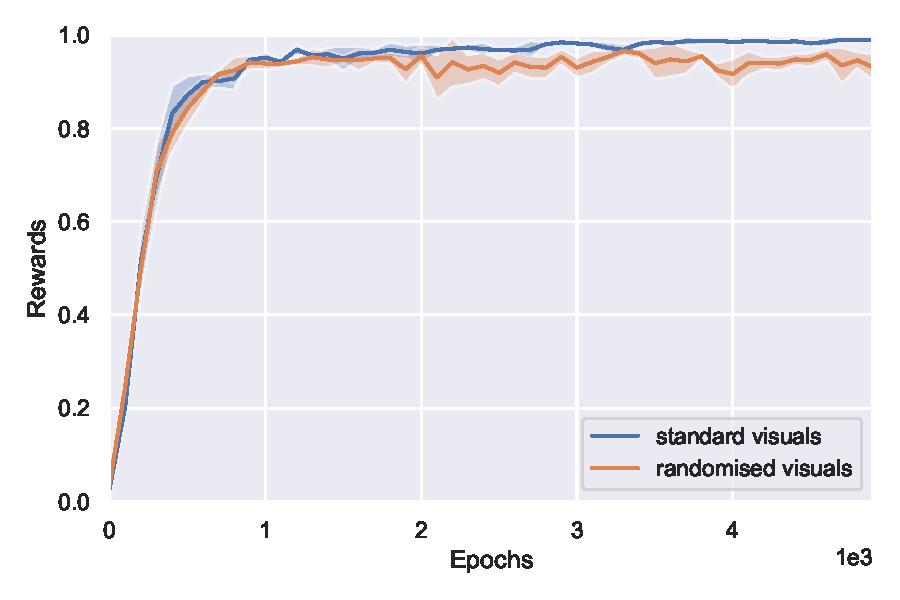
\includegraphics[width=\textwidth]{figures/chapter6/training_curves/jaco_prop.pdf}
    \caption{Proprioceptive inputs}
  \end{subfigure}
  \hfill
  \begin{subfigure}{0.45\textwidth}
    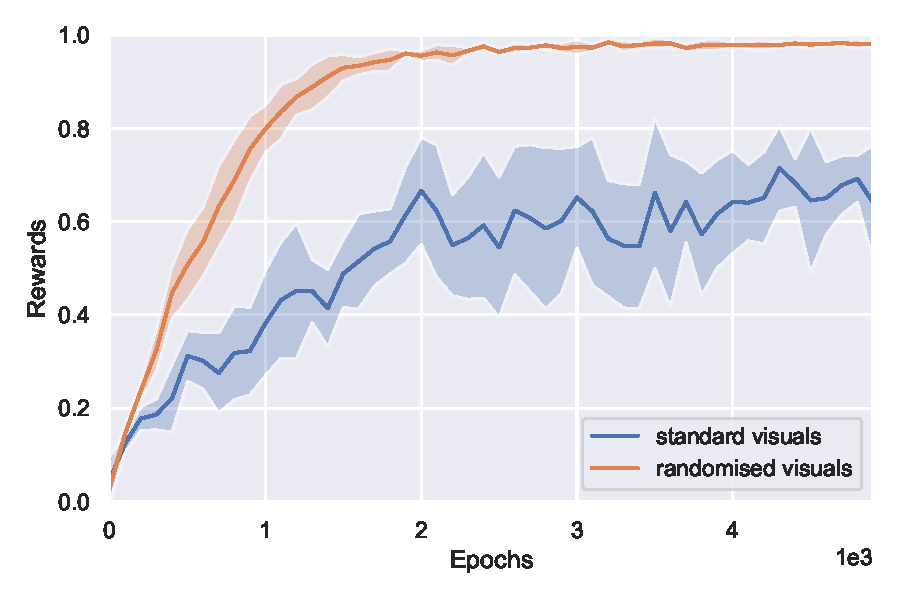
\includegraphics[width=\textwidth]{figures/chapter6/training_curves/jaco_noprop.pdf}
    \caption{No proprioceptive inputs}
  \end{subfigure}
  \hspace{0.025\textwidth}
  \caption{Test performance of Jaco agents trained with DR and (a) with or (b) without proprioceptive inputs; the agents are tested against both standard and randomised visuals. Without proprioceptive inputs, the agents fail to fully deal with the domain gap between the randomised and standard visuals. Statistics (median and 95\% confidence interval) are calculated over all models (seeds) and test target locations.}
  \label{fig:domain_shift}
\end{figure}

Once agents are successfully trained on each of the different conditions
(Fetch/Jaco, DR/no DR, proprioceptive/no proprioceptive inputs), we can
perform further tests to see how they generalise. However, while the
agents achieve practically perfect test performance on the conditions
that they were trained under, the Jaco agents trained with DR but
without proprioceptive inputs fare worse when tested under the
simulator's standard visuals (Figure \ref{fig:domain_shift}),
demonstrating a drop in performance under domain shift. It is both
assumed and observed that domain shift occurs when transferring models
trained with DR to the more complex and noisy visuals of the real world,
but it is somewhat unexpected to see this happen when shifting to
simpler visuals, which are expected to be a subset of DR visuals---this
indicates that the agent is in some way overfitting to the DR visuals.
Because of this, it is not completely straightforward to compare
performance between different agents, but the change in performance of a
single agent over differing test conditions is still highly meaningful.

We also trained agents with visual DR where the visuals were only
randomised at the beginning of each episode, and kept fixed during.
These agents exhibited the same gap in performance between the standard
and randomised visuals, indicating that this is not an issue of temporal
consistency in the DR setup. Therefore, while agents trained with visual
DR may be invariant to the visual conditions observed during training,
this invariance may have limited OoD generalisation with respect to
backgrounds (Figure \ref{fig:strategies}).

\hypertarget{test-scenarios}{%
\subsection{Test Scenarios}\label{test-scenarios}}

\label{sec:test_scenarios}

In order to test how the agents generalise to different held-out
conditions, we constructed a suite of tests for the trained agents
(Figure \ref{fig:tests} for observations for Fetch under the different
conditions\footnote{Simulation environment parameters of the Mujoco can
  be referenced from \url{http://www.mujoco.org/book/XMLreference.html}.},
and Table \ref{tbl:tests} for the results):

\begin{figure*}
  \centering
  \begin{subfigure}{0.19\textwidth}
    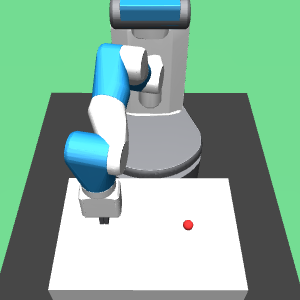
\includegraphics[width=\textwidth]{figures/chapter6/test_observations/standard}
    \caption{Standard}
  \end{subfigure}
  \begin{subfigure}{0.19\textwidth}
    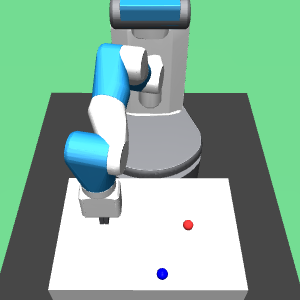
\includegraphics[width=\textwidth]{figures/chapter6/test_observations/colour_b}
    \caption{Colour}
  \end{subfigure}
  \begin{subfigure}{0.19\textwidth}
    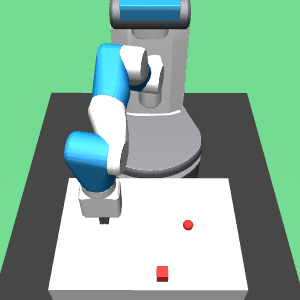
\includegraphics[width=\textwidth]{figures/chapter6/test_observations/shape}
    \caption{Shape}
  \end{subfigure}
  \begin{subfigure}{0.19\textwidth}
    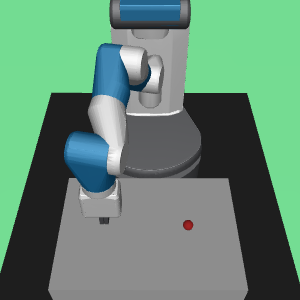
\includegraphics[width=\textwidth]{figures/chapter6/test_observations/illumination}
    \caption{Illumination (Lvl.)}
  \end{subfigure}
  \begin{subfigure}{0.19\textwidth}
    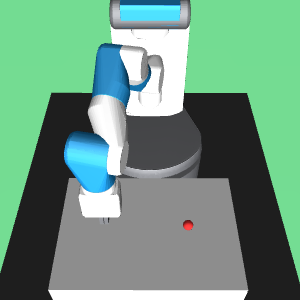
\includegraphics[width=\textwidth]{figures/chapter6/test_observations/illumination_dir}
    \caption{Illumination (Dir.)}
  \end{subfigure}

  \begin{subfigure}{0.19\textwidth}
    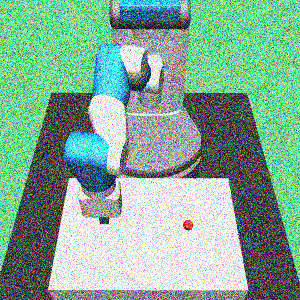
\includegraphics[width=\textwidth]{figures/chapter6/test_observations/noise}
    \caption{Noise}
  \end{subfigure}
  \begin{subfigure}{0.19\textwidth}
    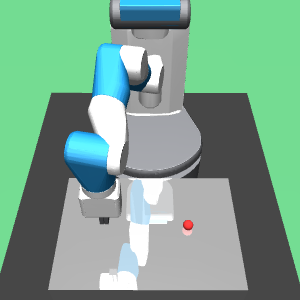
\includegraphics[width=\textwidth]{figures/chapter6/test_observations/reflection}
    \caption{Reflection}
  \end{subfigure}
  \begin{subfigure}{0.19\textwidth}
    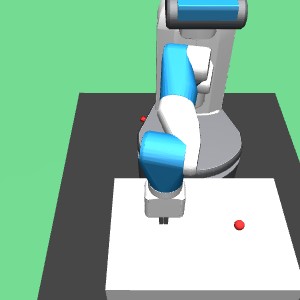
\includegraphics[width=\textwidth]{figures/chapter6/test_observations/translation}
    \caption{Translation}
  \end{subfigure}
  \begin{subfigure}{0.19\textwidth}
    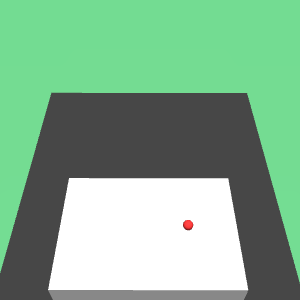
\includegraphics[width=\textwidth]{figures/chapter6/test_observations/invisible}
    \caption{Invisibility}
  \end{subfigure}
  \caption{Camera observations for Fetch under different test conditions.}
  \label{fig:tests}
\end{figure*}

\begin{description}
\item[Standard.] This is the standard evaluation procedure with the default simulator visuals, where the deterministic policy is applied to all test target positions and the performance is averaged (1.0 means that all targets were reached within 20 timesteps). 
\item[Colour.] This introduces a non-red sphere distractor object that is the same size and shape as the target. This tests the sensitivity of the policy to localising the target given another object of a different colour. We use yellow, blue, green, brown and purple; some of these colours have a red component (yellow, brown and purple), while others do not (blue and green).
\item[Shape.] This introduces a red distractor object that is the same width and colour as the target, but a different shape. We use a cube, ellipsoid, rectangle and diamond.
\item[Illumination (Lvl.).] This changes the diffuse colour of the main light. We use 5 illumination levels: 0.4 to 0.0 for Fetch, and 0.9 to 0.1 for Jaco.
\item[Illumination (Dir.).] This changes the location of the main light. We use 5 different directions for both robots. 
\item[Noise.] This adds Gaussian noise $\sim N(0, 0.25)$ to the visual observations. 
\item[Reflection.] This sets the table (for Fetch) or ground (for Jaco) to be reflective. This introduces reflections of the robot (and the target for Jaco) in the input.
\item[Translation.] This offsets the RGB camera. We use 5 locations: -20 to 20cm in the x direction for Jaco, and -20 to 20cm in the y direction for Fetch.
\item[Invisibility.] This makes the robot transparent; this is not a realistic alteration, but is instead used to test the importance of the visual inputs for self-localisation.
\end{description}

\begin{table*}
  \caption{Test performance of all models with local visual changes (distractors), global visual changes, and invisibility (visual self-localisation test). Colour and shape results are averaged over 9 different distractor locations, as well as all colours and shapes, respectively. Checkmarks and crosses indicate enabling/disabling DR and proprioceptive inputs (Prop.), respectively. Statistics are calculated over all models (seeds) and test target locations.}
  \label{tbl:tests}
  \resizebox{\linewidth}{!}{
  \begin{tabular}{c|cc|c|cc|cc|ccc|c}
    \toprule
    Robot & DR & Prop. & Standard & Colours & Shapes & Illumination (Lvl.) & Illumination (Dir.) & Noise & Reflection & Translation & Invisibility\\
    \midrule
    Fetch & \textcolor{red}{\xmark}   & \textcolor{red}{\xmark}   & 1.000$\pm 0.000$ & 0.993$\pm 0.004$ & 0.827$\pm 0.056$ & 0.694$\pm 0.049$ & 0.539$\pm 0.069$ & 0.980$\pm 0.006$ & 0.447$\pm 0.039$ & 0.270$\pm 0.079$ & 0.000$\pm 0.000$\\
    Fetch & \textcolor{red}{\xmark}   & \textcolor{green}{\cmark} & 1.000$\pm 0.000$ & 0.937$\pm 0.027$ & 0.524$\pm 0.087$ & 0.593$\pm 0.064$ & 0.491$\pm 0.066$ & 0.988$\pm 0.004$ & 0.570$\pm 0.078$ & 0.231$\pm 0.078$ & 0.000$\pm 0.000$\\
    Fetch & \textcolor{green}{\cmark} & \textcolor{red}{\xmark}   & 0.983$\pm 0.004$ & 0.974$\pm 0.004$ & 0.939$\pm 0.018$ & 0.957$\pm 0.008$ & 0.740$\pm 0.058$ & 0.985$\pm 0.007$ & 0.972$\pm 0.011$ & 0.480$\pm 0.064$ & 0.000$\pm 0.000$\\
    Fetch & \textcolor{green}{\cmark} & \textcolor{green}{\cmark} & 0.997$\pm 0.002$ & 0.997$\pm 0.001$ & 0.978$\pm 0.009$ & 0.992$\pm 0.002$ & 0.883$\pm 0.038$ & 0.970$\pm 0.008$ & 0.985$\pm 0.005$ & 0.536$\pm 0.063$ & 0.023$\pm 0.015$\\
    \hline
    Jaco  & \textcolor{red}{\xmark}   & \textcolor{red}{\xmark}   & 0.995$\pm 0.003$ & 0.772$\pm 0.058$ & 0.367$\pm 0.069$ & 0.966$\pm 0.012$ & 0.838$\pm 0.035$ & 0.635$\pm 0.028$ & 0.734$\pm 0.032$ & 0.556$\pm 0.063$ & 0.000$\pm 0.000$\\
    Jaco  & \textcolor{red}{\xmark}   & \textcolor{green}{\cmark} & 0.995$\pm 0.001$ & 0.808$\pm 0.044$ & 0.382$\pm 0.064$ & 0.876$\pm 0.032$ & 0.911$\pm 0.014$ & 0.478$\pm 0.059$ & 0.618$\pm 0.061$ & 0.688$\pm 0.048$ & 0.001$\pm 0.001$\\
    Jaco  & \textcolor{green}{\cmark} & \textcolor{red}{\xmark}   & 0.650$\pm 0.056$ & 0.652$\pm 0.022$ & 0.593$\pm 0.031$ & 0.643$\pm 0.027$ & 0.549$\pm 0.032$ & 0.575$\pm 0.040$ & 0.429$\pm 0.060$ & 0.310$\pm 0.041$ & 0.007$\pm 0.002$\\
    Jaco  & \textcolor{green}{\cmark} & \textcolor{green}{\cmark} & 0.991$\pm 0.004$ & 0.989$\pm 0.002$ & 0.843$\pm 0.061$ & 0.816$\pm 0.043$ & 0.882$\pm 0.031$ & 0.896$\pm 0.007$ & 0.946$\pm 0.006$ & 0.658$\pm 0.054$ & 0.916$\pm 0.022$\\
    \bottomrule
  \end{tabular}}
\end{table*}

\begin{table*}
  \caption{Test performance of all models with local visual changes (distractors). Checkmarks and crosses indicate enabling/disabling DR and proprioceptive inputs (Prop.), respectively. Statistics are calculated over all models (seeds), test target locations, and 9 distractor locations.}
  \label{tbl:diff_colours}
  \resizebox{\linewidth}{!}{
  \begin{tabular}{c|cc|ccccc|cccc}
    \toprule
    Robot & DR & Prop. & Yellow & Blue & Green & Brown & Purple & Cube & Ellipsoid & Rectangle & Diamond\\
    \midrule
    Fetch & \textcolor{red}{\xmark}   & \textcolor{red}{\xmark}   & 0.993$\pm 0.007$ & 1.000$\pm 0.000$ & 1.000$\pm 0.000$ & 0.978$\pm 0.017$ & 0.995$\pm 0.004$ & 0.775$\pm 0.085$ & 0.993$\pm 0.007$ & 0.960$\pm 0.036$ & 0.580$\pm 0.142$\\
    Fetch & \textcolor{red}{\xmark}   & \textcolor{green}{\cmark} & 0.875$\pm 0.088$ & 1.000$\pm 0.000$ & 1.000$\pm 0.000$ & 0.825$\pm 0.069$ & 0.983$\pm 0.006$ & 0.243$\pm 0.064$ & 0.980$\pm 0.006$ & 0.783$\pm 0.079$ & 0.090$\pm 0.048$\\
    Fetch & \textcolor{green}{\cmark} & \textcolor{red}{\xmark}   & 0.970$\pm 0.011$ & 0.980$\pm 0.006$ & 0.975$\pm 0.006$ & 0.973$\pm 0.010$ & 0.973$\pm 0.011$ & 0.913$\pm 0.042$ & 0.975$\pm 0.009$ & 0.965$\pm 0.013$ & 0.905$\pm 0.048$\\
    Fetch & \textcolor{green}{\cmark} & \textcolor{green}{\cmark} & 0.995$\pm 0.003$ & 0.998$\pm 0.002$ & 1.000$\pm 0.000$ & 0.998$\pm 0.002$ & 0.995$\pm 0.003$ & 0.963$\pm 0.020$ & 0.998$\pm 0.002$ & 0.995$\pm 0.003$ & 0.958$\pm 0.022$\\
    \hline
    Jaco  & \textcolor{red}{\xmark}   & \textcolor{red}{\xmark}   & 0.281$\pm 0.067$ & 0.871$\pm 0.036$ & 0.994$\pm 0.003$ & 0.730$\pm 0.095$ & 0.984$\pm 0.008$ & 0.274$\pm 0.077$ & 0.407$\pm 0.098$ & 0.759$\pm 0.066$ & 0.027$\pm 0.006$\\
    Jaco  & \textcolor{red}{\xmark}   & \textcolor{green}{\cmark} & 0.451$\pm 0.040$ & 0.941$\pm 0.032$ & 0.993$\pm 0.002$ & 0.706$\pm 0.064$ & 0.950$\pm 0.028$ & 0.258$\pm 0.044$ & 0.440$\pm 0.058$ & 0.784$\pm 0.044$ & 0.045$\pm 0.009$\\
    Jaco  & \textcolor{green}{\cmark} & \textcolor{red}{\xmark}   & 0.640$\pm 0.046$ & 0.655$\pm 0.055$ & 0.651$\pm 0.055$ & 0.668$\pm 0.046$ & 0.648$\pm 0.046$ & 0.636$\pm 0.040$ & 0.642$\pm 0.035$ & 0.666$\pm 0.047$ & 0.426$\pm 0.054$\\
    Jaco  & \textcolor{green}{\cmark} & \textcolor{green}{\cmark} & 0.987$\pm 0.005$ & 0.990$\pm 0.003$ & 0.987$\pm 0.003$ & 0.990$\pm 0.003$ & 0.990$\pm 0.003$ & 0.970$\pm 0.017$ & 0.970$\pm 0.011$ & 0.990$\pm 0.003$ & 0.441$\pm 0.128$\\
    \bottomrule
  \end{tabular}}
\end{table*}

\hypertarget{local-visual-changes}{%
\subsubsection{Local Visual Changes}\label{local-visual-changes}}

Noting that the baseline performance of the Jaco model trained with DR
but without proprioception is lower under standard visuals, across both
robots, DR confers robustness to both the colour and shape distractors
(Table \ref{tbl:tests}). However, there is not as consistent a pattern
between agents trained without DR. Table \ref{tbl:diff_colours} provides
an extended breakdown across the different colours and shapes, which
provides important information on what strategies the agents have
learned.

With Fetch, colour distractors have little effect on the agents, but the
shape distractor diminishes the performance of the non-DR agent trained
without proprioception somewhat, and the non-DR agent trained with
proprioception significantly. Given this, it seems that the latter agent
relies mainly on detecting \emph{pure} red (plus some shape information)
in order to locate the ball. As a result of self-localising based on
visual input alone, the former agent develops more sophisticated vision,
allowing the model to better distinguish both shapes and colours.

With Jaco, both non-DR agents suffer noticeable drops in performance in
the presence of distractors with a red component, whilst both DR agents
experience only a very small decrease in performance across all local
distractors (bar the diamond, which looks the most similar to a sphere,
especially at lower resolutions). While the non-DR agents also have
reduced success with the blue sphere distractor, it is less pronounced,
indicating that non-DR Jaco agents are primarily detecting large red
components as the target object.

In order to test that the location of the distractor does not also
influence the models' responses, we varied this and recorded the
corresponding success rates. The low standard deviations shown in Table
\ref{tbl:vary_distractor} indicate that the location only has a minimal
impact on the results.

\hypertarget{global-visual-changes}{%
\subsubsection{Global Visual Changes}\label{global-visual-changes}}

Referring to Table \ref{tbl:tests}, DR generally confers more
robustness, although this time the DR agents do exhibit noticeable drops
in performance across many of these tests.

Reducing the illumination levels drops the performance of all agents
monotonically with respect to dimness (Table \ref{tbl:diff_levels}),
although the Fetch agents trained with DR are the most robust.
Intriguingly, the Jaco agents trained without proprioception are more
robust with respect to this change, as compared to the agents trained
with. Their need to self-localise visually necessitates a more complex
visual system, whereas simpler visual processing may be thrown off by
the reduction in contrast or even simply the change in the pixel values
of the target. Given that the DR agents trained with proprioception tend
to be the most robust across most of the test conditions, this motivates
an additional consideration for training---when performing sensor fusion
within a model, the combination of information should be more resilient
to the loss or faulty functioning of any individual sensory input.

Changing the direction of the main illumination degrades the performance
of all agents. As before, Fetch agents trained with DR are more robust
than those trained without, but for Jaco agents the presence of
proprioceptive inputs are more important than training with DR. This
trend holds across different illumination directions (Table
\ref{tbl:diff_dirs}).

Additive Gaussian noise has very little effect on the Fetch agents, but
reduces the performance of the Jaco agents---by over 30\% for agents
trained without DR, but only by about 10\% for agents trained with DR.
Considering other factors are consistent across training conditions,
either the visual layout or difficulty of the task caused the Fetch
agents to be more robust to noise than the Jaco agents.

Making the table surface reflective throws off the Fetch agents trained
without DR, with an approximately 50\% drop in performance, but with DR
the agents are resilient to this change. The Jaco agents trained without
DR also incur a significant, yet smaller drop in performance. A likely
explanation for this difference is that the size of the robots relative
to the image differs, and the reflection of the Jaco arm simply changes
the input less. When given proprioceptive inputs, both the Fetch and the
Jaco agent trained with DR display similar levels of resilience.

Translating the camera causes a dramatic drop in performance in all
agents. DR confers some amount of resilience to this for the Fetch
agents. However, all Jaco agents are similarly affected, DR or not, and
their average success rates are higher than those of the Fetch agents.
This suggests that all Jaco agents manage to learn a degree of
translation invariance for their policies. One hypothesis for this is
that the requirement to reach a target in 3D confers a more
generalisable representation of space. Performance drops monotonically
with deviation from the original location (Table \ref{tbl:diff_trans}).
The drop is symmetric for the Fetch agents, but asymmetric for the Jaco
agents---a relative shift in the target towards the centre of the image
input is better than a shift away.

\hypertarget{visual-self-localisation}{%
\subsubsection{Visual
Self-localisation}\label{visual-self-localisation}}

\label{sec:vis_self_loc}

For nearly all agents, rendering the robot invisible drops performance
to zero. There are four non-zero performance scores, but three of these
are low enough to be attributable to chance. This test indicates that
perhaps either directly or indirectly the position of the robot is
inferred visually, although we cannot rule out that the drop in
performance is due to the domain shift that results from rendering the
arm invisible. The standout is the Jaco agent with proprioceptive inputs
and DR training, which only incurs a small drop in performance---this
agent is able to self-localise solely based on proprioceptive input.

\hypertarget{tests-summary}{%
\subsubsection{Tests Summary}\label{tests-summary}}

\begin{figure}
  \centering
  \begin{subfigure}{0.45\textwidth}
    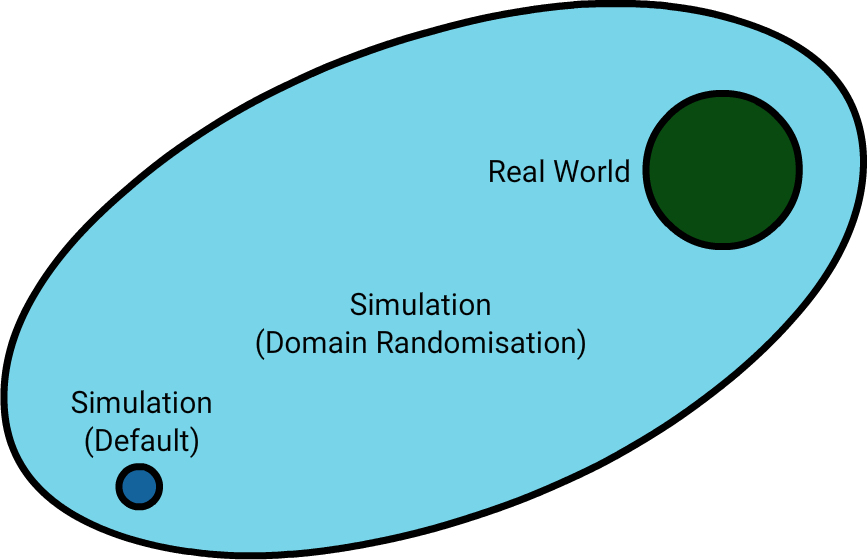
\includegraphics[width=\linewidth]{figures/chapter6/dr_concept}
    \subcaption{Idealised theory}
  \end{subfigure}
  \hspace{0.05\textwidth}
  \begin{subfigure}{0.45\textwidth}
    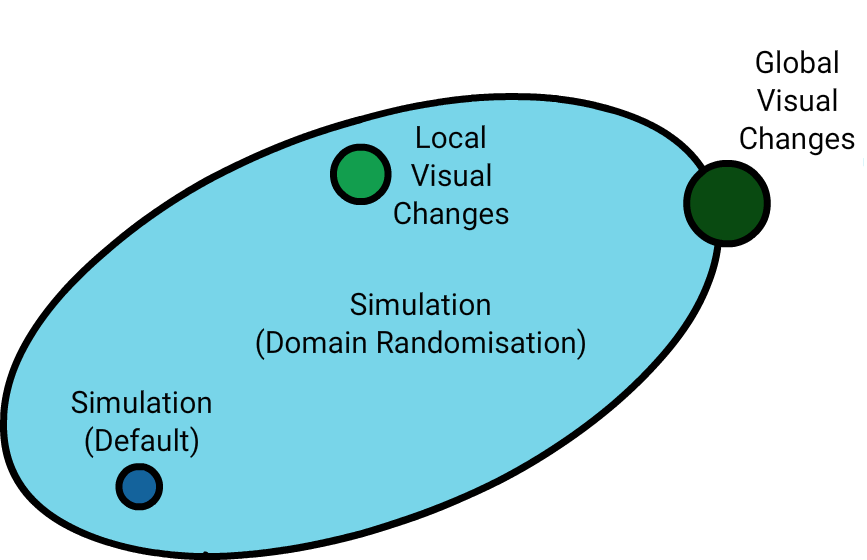
\includegraphics[width=\linewidth]{figures/chapter6/dr_concept_results}
    \subcaption{Our experiments for testing OoD generalisation}
  \end{subfigure}
  \caption[Domain randomisation methodology.]{Domain randomisation methodology. (a) In theory, the range of simulation parameters should be varied in such a way as to successfully encompass visual/physical properties that would be encountered in the real world. (b) In practice, we limited the scope of variation to test generalisation to OoD inputs within simulation, and observed different levels of success depending on the type of change; depending on the training settings we even observe some level of overfitting. The local and global visual changes in our tests are designed to evaluate generalisation in a way that is reflective of the real world.}
  \label{fig:dr_concept}
\end{figure}

There is no single clear result from our evaluation of different setups
with different types of tests, beyond the general importance of sensor
fusion and DR to improve the ability for agents to generalise. The type
of DR used during training---randomising colours and textures---allows
generalisation to localised changes---distractor objects---but fails to
reliably improve generalisation across the more global changes, such as
illumination or translation (Figure \ref{fig:dr_concept}). This should
not come as a surprise given that our DR never changed the position of
the robot, nor the illumination of the target. The takeaway is that
``generalisation'' is more nuanced, and performing systematic tests can
help probe what strategies networks might be using to operate. Finding
failure cases for ``weaker'' agents can still be a useful exercise for
evaluating more robust agents, as it enables adversarial evaluation
\cite{uesato2018rigorous}, and can inform us about the design of DR.

\hypertarget{model-analysis}{%
\section{Model Analysis}\label{model-analysis}}

\label{sec:model_analysis}

The unit tests that we constructed can be used to evaluate the
performance of an arbitrary black box policy under differing conditions,
but we also have the ability to inspect the internals of our trained
agents. Although we cannot obtain a complete explanation for the learned
policies, we can still glean further information from both the learned
parameters and the sets of activations in the networks.

\hypertarget{saliency-maps-1}{%
\subsection{Saliency Maps}\label{saliency-maps-1}}

\label{sec:saliency_maps}

One of the first tests usually conducted is to examine saliency maps to
infer which aspects of the input influence the output of the agent. We
use the occlusion-based technique with average baseline, and focus on
distractors: we show saliency maps for both the standard test setup, and
with either the different colour (yellow) or different shape (cube)
distractors.

\begin{figure}
  \centering
  \begin{subfigure}{0.24\columnwidth}
    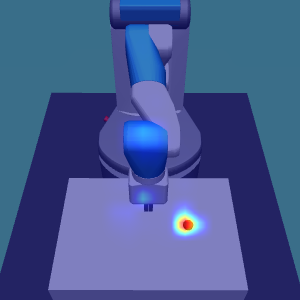
\includegraphics[width=\linewidth]{figures/chapter6/distractor_saliency_fetch_pro_off/standard_visual_std}
    \subcaption{Standard (no DR, no proprioception)}
  \end{subfigure}
  \begin{subfigure}{0.24\columnwidth}
    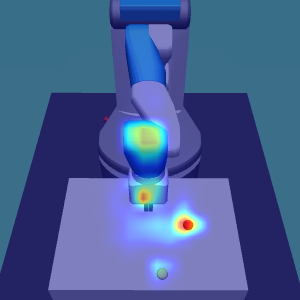
\includegraphics[width=\linewidth]{figures/chapter6/distractor_saliency_fetch_pro_off/color_visual_std}
    \subcaption{Colour (no DR, no proprioception)}
  \end{subfigure}
  \begin{subfigure}{0.24\columnwidth}
    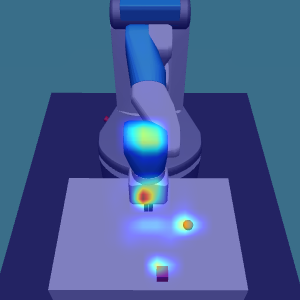
\includegraphics[width=\linewidth]{figures/chapter6/distractor_saliency_fetch_pro_off/shape_visual_std}
    \subcaption{Shape (no DR, no proprioception)}
  \end{subfigure}
  \begin{subfigure}{0.24\columnwidth}
    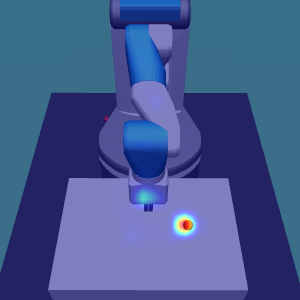
\includegraphics[width=\linewidth]{figures/chapter6/distractor_saliency_fetch_pro_on/standard_sensor_std}
    \subcaption{Standard (no DR, proprioception)}
  \end{subfigure}
  
  \begin{subfigure}{0.24\columnwidth}
    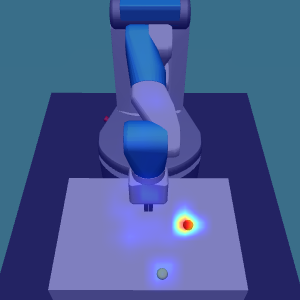
\includegraphics[width=\linewidth]{figures/chapter6/distractor_saliency_fetch_pro_on/color_sensor_std}
    \subcaption{Colour (no DR, proprioception)}
  \end{subfigure}
  \begin{subfigure}{0.24\columnwidth}
    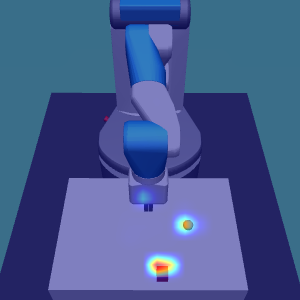
\includegraphics[width=\linewidth]{figures/chapter6/distractor_saliency_fetch_pro_on/shape_sensor_std}
    \subcaption{Shape (no DR, proprioception)}
  \end{subfigure}
  \begin{subfigure}{0.24\columnwidth}
    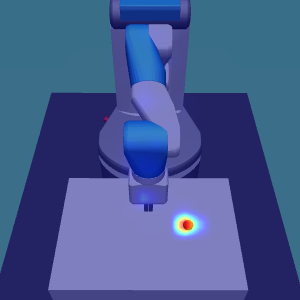
\includegraphics[width=\linewidth]{figures/chapter6/distractor_saliency_fetch_pro_off/standard_visual_random}
    \subcaption{Standard (DR, no proprioception)}
  \end{subfigure}
  \begin{subfigure}{0.24\columnwidth}
    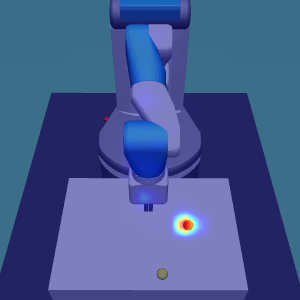
\includegraphics[width=\linewidth]{figures/chapter6/distractor_saliency_fetch_pro_off/color_visual_random}
    \subcaption{Colour (DR, no proprioception)}
  \end{subfigure}
  
  \begin{subfigure}{0.24\columnwidth}
    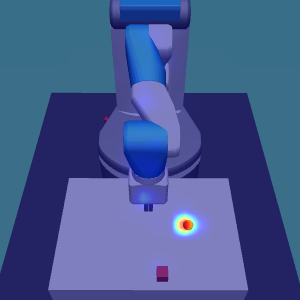
\includegraphics[width=\linewidth]{figures/chapter6/distractor_saliency_fetch_pro_off/shape_visual_random}
    \subcaption{Shape (DR, no proprioception)}
  \end{subfigure}
  \begin{subfigure}{0.24\columnwidth}
    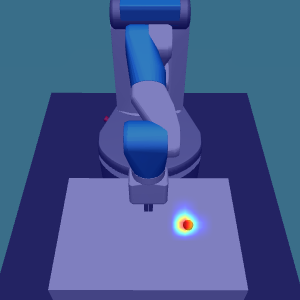
\includegraphics[width=\linewidth]{figures/chapter6/distractor_saliency_fetch_pro_on/standard_sensor_random}
    \subcaption{Standard (DR, proprioception)}
  \end{subfigure}
  \begin{subfigure}{0.24\columnwidth}
    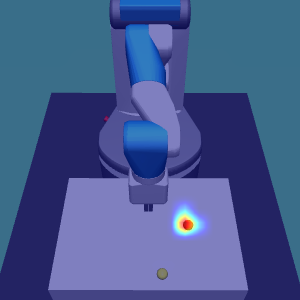
\includegraphics[width=\linewidth]{figures/chapter6/distractor_saliency_fetch_pro_on/color_sensor_random}
    \subcaption{Colour (DR, proprioception)}
  \end{subfigure}
  \begin{subfigure}{0.24\columnwidth}
    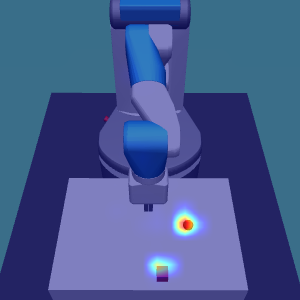
\includegraphics[width=\linewidth]{figures/chapter6/distractor_saliency_fetch_pro_on/shape_sensor_random}
    \subcaption{Shape (DR, proprioception)}
  \end{subfigure}
  \caption{Occlusion-based saliency maps with Fetch models trained with (g-l) or without (a-f) DR and with (d-f, j-l) or without proprioception (a-c, g-i) in three different distractor conditions. The best Fetch model was used for each training condition.}
  \label{fig:saliency_fetch_distractor}
\end{figure}

\begin{figure*}
  \centering
  \begin{subfigure}{0.24\columnwidth}
    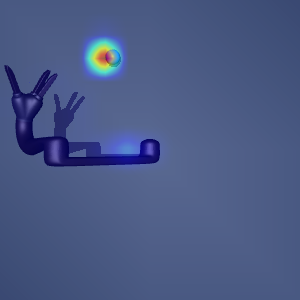
\includegraphics[width=\linewidth]{figures/chapter6/distractor_saliency_jaco_pro_off/standard_visual_std}
    \subcaption{Standard (no DR, no proprioception)}
  \end{subfigure}
  \begin{subfigure}{0.24\columnwidth}
    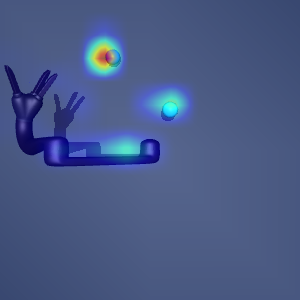
\includegraphics[width=\linewidth]{figures/chapter6/distractor_saliency_jaco_pro_off/color_visual_std}
    \subcaption{Colour (no DR, no proprioception)}
  \end{subfigure}
  \begin{subfigure}{0.24\columnwidth}
    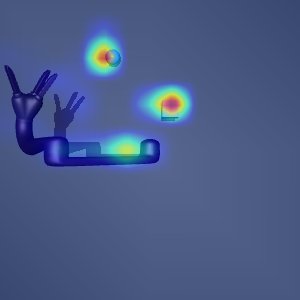
\includegraphics[width=\linewidth]{figures/chapter6/distractor_saliency_jaco_pro_off/shape_visual_std}
    \subcaption{Shape (no DR, no proprioception)}
  \end{subfigure}
  \begin{subfigure}{0.24\columnwidth}
    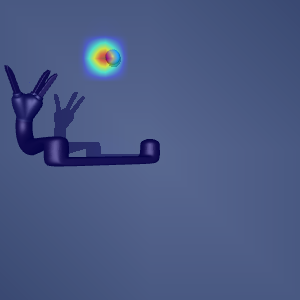
\includegraphics[width=\linewidth]{figures/chapter6/distractor_saliency_jaco_pro_on/standard_sensor_std}
    \subcaption{Standard (no DR, proprioception)}
  \end{subfigure}
  
  \begin{subfigure}{0.24\columnwidth}
    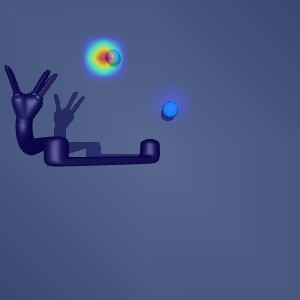
\includegraphics[width=\linewidth]{figures/chapter6/distractor_saliency_jaco_pro_on/color_sensor_std}
    \subcaption{Colour (no DR, proprioception)}
  \end{subfigure}
  \begin{subfigure}{0.24\columnwidth}
    \includegraphics[width=\linewidth]{figures/chapter6/distractor_saliency_jaco_pro_on/shape_sensor_std}
    \subcaption{Shape (no DR, proprioception)}
  \end{subfigure}
  \begin{subfigure}{0.24\columnwidth}
    \includegraphics[width=\linewidth]{figures/chapter6/distractor_saliency_jaco_pro_off/standard_visual_random}
    \subcaption{Standard (DR, no proprioception)}
  \end{subfigure}
  \begin{subfigure}{0.24\columnwidth}
    \includegraphics[width=\linewidth]{figures/chapter6/distractor_saliency_jaco_pro_off/color_visual_random}
    \subcaption{Colour (DR, no proprioception)}
  \end{subfigure}
  
  \begin{subfigure}{0.24\columnwidth}
    \includegraphics[width=\linewidth]{figures/chapter6/distractor_saliency_jaco_pro_off/shape_visual_random}
    \subcaption{Shape (DR, no proprioception)}
  \end{subfigure}
  \begin{subfigure}{0.24\columnwidth}
    \includegraphics[width=\linewidth]{figures/chapter6/distractor_saliency_jaco_pro_on/standard_sensor_random}
    \subcaption{Standard (DR, proprioception)}
  \end{subfigure}
  \begin{subfigure}{0.24\columnwidth}
    \includegraphics[width=\linewidth]{figures/chapter6/distractor_saliency_jaco_pro_on/color_sensor_random}
    \subcaption{Colour (DR, proprioception)}
  \end{subfigure}
  \begin{subfigure}{0.24\columnwidth}
    \includegraphics[width=\linewidth]{figures/chapter6/distractor_saliency_jaco_pro_on/shape_sensor_random}
    \subcaption{Shape (DR, proprioception)}
  \end{subfigure}
  \caption{Occlusion-based saliency maps with Jaco models trained with (g-l) or without (a-f) DR and with (d-f, j-l) or without proprioception (a-c, g-i) in three different distractor conditions. The best Jaco model was used for each training condition.}
  \label{fig:saliency_jaco_distractor}
\end{figure*}

The saliency maps for the Fetch agents (Figure
\ref{fig:saliency_fetch_distractor}) differ between all models. Apart
from the model trained with DR and with proprioception (Figure
\ref{fig:saliency_fetch_distractor}j-l), all agents seem to use the
gripper to self-localise. Despite having access to clean proprioceptive
inputs, the Fetch agent trained without DR still pays attention to its
own body in the image (i.e., visual localisation strategy; Figure
\ref{fig:strategies})---so it is not necessarily the case that agents
will even utilise the inputs that we may expect. The Fetch agents
trained without DR show saliency on the distractors (Figure
\ref{fig:saliency_fetch_distractor}a-f), while the agents trained with
DR do not (with the exception of the model trained with DR and
proprioception on the shape distractor, as seen in Figure
\ref{fig:saliency_fetch_distractor}).

The saliency maps for the Jaco agents (Figure
\ref{fig:saliency_jaco_distractor}) are more homogeneous, with a large
amount of attention on the target, and little elsewhere. The saliency
for the agent trained without DR and without proprioception clearly
shows some attention around the base of the arm (Figure
\ref{fig:saliency_jaco_distractor}a-c) that would indicate visual
self-localisation. On an initial inspection, it may appear that there is
no saliency around the arm for the agent trained with DR and without
proprioception, although we know that in order to succeed it must be
relying on visual self-localisation. Indeed, there is saliency present
around the arm (Figure \ref{fig:saliency_jaco_distractor}g-i), but it is
difficult to perceive. This example indicates the subjective nature of
interpreting saliency maps, and hence why they should not be the sole
tool for analysis.

This recommendation is also borne out by the mismatch between the
saliency maps and performance. For the Fetch agents trained with DR, the
agent with proprioception shows saliency over the shape distractor
(Figure \ref{fig:saliency_fetch_distractor}l) in contrast to without
proprioception (Figure \ref{fig:saliency_fetch_distractor}i);
conversely, the performance drop is greater in the latter than the
former (Table \ref{tbl:diff_colours}). Similarly for the Jaco agents
trained without DR, the agent without proprioception shows a large
amount of saliency over the shape distractor (Figure
\ref{fig:saliency_jaco_distractor}c), while the agent with
proprioception demonstrates only a minimal amount of saliency (Figure
\ref{fig:saliency_jaco_distractor}f); however, they both have a similar
drop in performance (Table \ref{tbl:diff_colours}).

\hypertarget{activation-maximisation-1}{%
\subsection{Activation Maximisation}\label{activation-maximisation-1}}

\label{sec:activation_maximisation}

\begin{figure}
  \centering
  \begin{subfigure}{0.49\textwidth}
    \includegraphics[width=\textwidth]{figures/chapter6/act_max/fetch_nodr_noprop_conv1}
    \caption{Convolution 1 (no DR, no proprioception)}
  \end{subfigure}
  \begin{subfigure}{0.49\textwidth}
    \includegraphics[width=\textwidth]{figures/chapter6/act_max/fetch_nodr_prop_conv1}
    \caption{Convolution 1 (no DR, proprioception)}
  \end{subfigure}

  \begin{subfigure}{0.49\textwidth}
    \includegraphics[width=\textwidth]{figures/chapter6/act_max/fetch_dr_noprop_conv1}
    \caption{Convolution 1 (DR, no proprioception)}
  \end{subfigure}
  \begin{subfigure}{0.49\textwidth}
    \includegraphics[width=\textwidth]{figures/chapter6/act_max/fetch_dr_prop_conv1}
    \caption{Convolution 1 (DR, proprioception)}
  \end{subfigure}

  \begin{subfigure}{0.49\textwidth}
    \includegraphics[width=\textwidth]{figures/chapter6/act_max/fetch_nodr_noprop_conv2}
    \caption{Convolution 2 (no DR, no proprioception)}
  \end{subfigure}
  \begin{subfigure}{0.49\textwidth}
    \includegraphics[width=\textwidth]{figures/chapter6/act_max/fetch_nodr_prop_conv2}
    \caption{Convolution 2 (no DR, proprioception)}
  \end{subfigure}

  \begin{subfigure}{0.49\textwidth}
    \includegraphics[width=\textwidth]{figures/chapter6/act_max/fetch_dr_noprop_conv2}
    \caption{Convolution 2 (DR, no proprioception)}
  \end{subfigure}
  \begin{subfigure}{0.49\textwidth}
    \includegraphics[width=\textwidth]{figures/chapter6/act_max/fetch_dr_prop_conv2}
    \caption{Convolution 2 (DR, proprioception)}
  \end{subfigure}
  
  \begin{subfigure}{0.49\textwidth}
    \centering
    \includegraphics[width=0.63\textwidth]{figures/chapter6/act_max/fetch_nodr_noprop_value_policy}
    \caption{Value + Policy (no DR, no proprioception)}
  \end{subfigure}
  \begin{subfigure}{0.49\textwidth}
    \centering
    \includegraphics[width=0.63\textwidth]{figures/chapter6/act_max/fetch_nodr_prop_value_policy}
    \caption{Value + Policy (no DR, proprioception)}
  \end{subfigure}

  \begin{subfigure}{0.49\textwidth}
    \centering
    \includegraphics[width=0.63\textwidth]{figures/chapter6/act_max/fetch_dr_noprop_value_policy}
    \caption{Value + Policy (DR, no proprioception)}
  \end{subfigure}
  \begin{subfigure}{0.49\textwidth}
    \centering
    \includegraphics[width=0.63\textwidth]{figures/chapter6/act_max/fetch_dr_prop_value_policy}
    \caption{Value + Policy (DR, proprioception)}
  \end{subfigure}
  \caption{Activation maximisation for trained Fetch agents: first convolutional layer (a-d); second convolutional layer (e-h); value and policy outputs (i-l). The best Fetch model was used for each training condition. Proprioceptive inputs and hidden state for value and policy visualisations are set to zero. Agents trained without DR have many red filters (the colour of the target) in the second layer (e, f), while agents trained with DR have more structured oriented red-blue filters (g, h). In comparison, the Jaco task induces more structured filters even without DR (see Figure \ref{fig:act_max_jaco}).}
  \label{fig:act_max_fetch}
\end{figure}

\begin{figure}
  \centering
  \begin{subfigure}{0.49\textwidth}
    \includegraphics[width=\textwidth]{figures/chapter6/act_max/jaco_nodr_noprop_conv1}
    \caption{Convolution 1 (no DR, no proprioception)}
  \end{subfigure}
  \begin{subfigure}{0.49\textwidth}
    \includegraphics[width=\textwidth]{figures/chapter6/act_max/jaco_nodr_prop_conv1}
    \caption{Convolution 1 (no DR, proprioception)}
  \end{subfigure}

  \begin{subfigure}{0.49\textwidth}
    \includegraphics[width=\textwidth]{figures/chapter6/act_max/jaco_dr_noprop_conv1}
    \caption{Convolution 1 (DR, no proprioception)}
  \end{subfigure}
  \begin{subfigure}{0.49\textwidth}
    \includegraphics[width=\textwidth]{figures/chapter6/act_max/jaco_dr_prop_conv1}
    \caption{Convolution 1 (DR, proprioception)}
  \end{subfigure}

  \begin{subfigure}{0.49\textwidth}
    \includegraphics[width=\textwidth]{figures/chapter6/act_max/jaco_nodr_noprop_conv2}
    \caption{Convolution 2 (no DR, no proprioception)}
  \end{subfigure}
  \begin{subfigure}{0.49\textwidth}
    \includegraphics[width=\textwidth]{figures/chapter6/act_max/jaco_nodr_prop_conv2}
    \caption{Convolution 2 (no DR, proprioception)}
  \end{subfigure}

  \begin{subfigure}{0.49\textwidth}
    \includegraphics[width=\textwidth]{figures/chapter6/act_max/jaco_dr_noprop_conv2}
    \caption{Convolution 2 (DR, no proprioception)}
  \end{subfigure}
  \begin{subfigure}{0.49\textwidth}
    \includegraphics[width=\textwidth]{figures/chapter6/act_max/jaco_dr_prop_conv2}
    \caption{Convolution 2 (DR, proprioception)}
  \end{subfigure}

  \begin{subfigure}{0.49\textwidth}
    \includegraphics[width=\textwidth]{figures/chapter6/act_max/jaco_nodr_noprop_value_policy}
    \caption{Value + Policy (no DR, no proprioception)}
  \end{subfigure}
  \begin{subfigure}{0.49\textwidth}
    \includegraphics[width=\textwidth]{figures/chapter6/act_max/jaco_nodr_prop_value_policy}
    \caption{Value + Policy (no DR, proprioception)}
  \end{subfigure}

  \begin{subfigure}{0.49\textwidth}
    \includegraphics[width=\textwidth]{figures/chapter6/act_max/jaco_dr_noprop_value_policy}
    \caption{Value + Policy (DR, no proprioception)}
  \end{subfigure}
  \begin{subfigure}{0.49\textwidth}
    \includegraphics[width=\textwidth]{figures/chapter6/act_max/jaco_dr_prop_value_policy}
    \caption{Value + Policy (DR, proprioception)}
  \end{subfigure}
  \caption{Activation maximisation for trained Jaco agents: first convolutional layer (a-d); second convolutional layer (e-h); value and policy outputs (i-l). The best Jaco model was used for each training condition. Proprioceptive inputs and hidden state for value and policy visualisations are set to zero. All agents have colour-gradient filters in the second layer (e-h), indicating more visual complexity than needed for the Fetch task (Figure \ref{fig:act_max_fetch}).}
  \label{fig:act_max_jaco}
\end{figure}

In line with Such et al. \cite{such2018atari}, activation maximisation
applied to the first convolutional layer results in edge detectors, with
larger-scale spatial structure in the latter layers (Figure
\ref{fig:act_max_fetch} and Figure \ref{fig:act_max_jaco}). There are
several trends that apply to both the Fetch and Jaco agents. Firstly,
the agents trained without DR develop simpler, more colourful filters in
both layers. In contrast, the agents trained with DR develop more
edge-like detectors, with higher contrast, in their first convolutional
layers. In their second convolutional layers, the feature detectors
resemble the red target itself, surrounded by a complementary
blue-green. This style of detector is consistent across both the
DR-trained Fetch and Jaco agents, which suggests that it was not
developed in response to the green floor in the Jaco environment. One
noticeable difference between the second set of convolutional filters
between the Fetch (Figure \ref{fig:act_max_fetch}g,h and Jaco (Figure
\ref{fig:act_max_jaco}g,h) agents is that the latter also develop
positional sensitivity, indicating that target localisation may be more
difficult.

The Jaco agent trained without DR and without proprioceptive inputs has
convolutional filters that respond maximally to yellow (Figure
\ref{fig:act_max_jaco}b), and is also the most affected by the yellow
distractor, with performance dropping to 28\% (Table
\ref{tbl:diff_colours}). Therefore this agent has learned a
ball-localisation strategy that is not purely based on detecting red or
spherical objects (Figure \ref{fig:strategies}).

Finally, there is a more global, but largely uninterpretable structure
when maximising the value function or policy outputs (choosing the unit
that corresponds to the largest positive movement per action output).
For Fetch agents without DR, the visualisations are dominated by red
(the target colour), but with DR there is a wider spectrum of colours.
This trend is the same for the Jaco agents, although without DR and
without proprioceptive inputs the colours that maximise the value output
are purple and green (a constant hue shift on the usual red and blue).
The agents trained with DR but without proprioception have the most
plain activation maximisation images for the policy, perhaps suggesting
a more factorised control scheme. For the Jaco agent (Figure
\ref{fig:act_max_jaco}k), only the first and third actuators are
activated by strong visual inputs (given zeroes as the proprioceptive
inputs and hidden state), which correspond to the most important joints
for accomplishing this reaching task (the rotating base and the elbow).

As a reminder we note that activation maximisation may not (and is
practically unlikely to) converge to images within the training data
manifold \cite{mahendran2015understanding}---a disadvantage addressed
by the complementary technique of finding image patches within the
training data that maximally activate individual neurons
\cite{girshick2014rich}. {Alternatively, one could train a generative model on the state distribution and query this model to generate novel states of interest}
\cite{olson2021counterfactual, rupprecht2020finding}.

\hypertarget{statistical-and-structural-weight-characterisations-1}{%
\subsection{Statistical and Structural Weight
Characterisations}\label{statistical-and-structural-weight-characterisations-1}}

\label{sec:statistical_and_structural}

\begin{figure*}
  \centering
  \begin{subfigure}{0.24\textwidth}
    \includegraphics[width=\textwidth]{figures/chapter6/weightdistributions/conv1_l1}
    \caption{$\ell_1$-norm (layer 1)}
  \end{subfigure}
  \begin{subfigure}{0.24\textwidth}
    \includegraphics[width=\textwidth]{figures/chapter6/weightdistributions/conv2_l1}
    \caption{$\ell_1$-norm (layer 2)}
  \end{subfigure}
  \begin{subfigure}{0.24\textwidth}
    \includegraphics[width=\textwidth]{figures/chapter6/weightdistributions/conv1_se}
    \caption{PSE (layer 1)}
  \end{subfigure}
  \begin{subfigure}{0.24\textwidth}
    \includegraphics[width=\textwidth]{figures/chapter6/weightdistributions/conv2_se}
    \caption{PSE (layer 2)}
  \end{subfigure}
  \caption{Effect of DR on statistical and structural characterisiations of convolutional filters, using all filters from all models, along with models with randomly initialised weights. This effect is layer-dependent, with a large change in $\ell_1$-norm for layer 2, but not layer 1, and a relatively larger change in PSE for layer 1 as compared to layer 2.}
  \label{fig:norms_entropy}
\end{figure*}

We calculated statistical and structural weight characteristics over all
trained models (Fetch and Jaco, with/without proprioception,
with/without DR, 5 seeds), which allows us to average over 40 conditions
to examine the effects of DR. We analysed the norms (Subsection
\ref{sec:magnitude}) of all of the weights of the trained agents, and
could not find consistent trends across all layers. The most meaningful
characterisations were the \(\ell_1\)-norm and the power spectral
entropy, PSE, (Subsection \ref{sec:spectral}), applied to the
convolutional filters.

Figure \ref{fig:norms_entropy} shows a KDE of the \(\ell_1\)-norms and
PSEs of all of the 2D filters within the first and second convolutional
layers. For the \(\ell_1\)-norm, in layer 2 the distribution is skewed
towards higher values when the model is trained with DR. For the PSE, in
both layers, but particularly layer 1, the distribution is skewed
towards lower values when the model is trained with DR. Using the
nonparametric Kolmogorov-Smirnov (K-S) two-sided test between the two
distributions (DR versus non-DR), the \(p\)-value of the
\(\ell_1\)-norms is 0.014 (K-S statistic 0.072) for layer 1 and
\(\sim 0\) (K-S statistic 0.285) for layer 2, and the \(p\)-value of the
PSEs is \(5.71\times10^{-27}\) (K-S statistic 0.251) for layer 1 and
\(3.32\times10^{-9}\) (K-S statistic 0.044) for layer 2. Given the same
weight initialisation distributions across all models, this difference
indicates that DR causes a significant change in the final distribution
of weights, with both larger weights and greater spatial structure.

\hypertarget{unit-ablations-1}{%
\subsection{Unit Ablations}\label{unit-ablations-1}}

\label{sec:unit_ablations}

\begin{figure*}
  \centering
  \begin{subfigure}{0.49\linewidth}
    \includegraphics[width=\textwidth]{figures/chapter6/unitablation/conv1_ablations}
    \caption{Standard environment (layer 1)}
  \end{subfigure}
  \begin{subfigure}{0.49\linewidth}
    \includegraphics[width=\textwidth]{figures/chapter6/unitablation/conv1_ablations_noisy}
    \caption{Noisy environment (layer 1)}
  \end{subfigure}

  \begin{subfigure}{0.49\linewidth}
    \includegraphics[width=\textwidth]{figures/chapter6/unitablation/conv2_ablations}
    \caption{Standard environment (layer 2)}
  \end{subfigure}
  \begin{subfigure}{0.49\linewidth}
    \includegraphics[width=\textwidth]{figures/chapter6/unitablation/conv2_ablations_noisy}
    \caption{Noisy environment (layer 2)}
  \end{subfigure}
  \caption{Unit-wise ablation tests in two different visual test environments. Each point corresponds to one unit in layer 1 (a, b) or layer 2 (c, d), with the vertical bars representing baseline performance in the test environment. The training settings correspond to the Fetch (F) and Jaco (J) robots, whether additional proprioceptive inputs are available (Prop), and if DR was used. The best model was used for each training condition. Note that the Jaco agent trained with DR but without proprioception already has a lower base performance on the standard visuals than the other models (Table \ref{tbl:tests}).}
  \label{fig:ablations}
\end{figure*}

Given access to the trained models, unit ablations allow us to perform a
quantitative, white box analysis. To ablate units, we manually zero the
activations of one of the output channels in either the first or second
convolutional layers, iterating the process over every channel. We then
re-evaluate the modified agents for each of the 8 training settings,
using the agent with the best performance over all 5 seeds for each one
(noting that the performance of the best Jaco agent trained with DR and
without proprioception is significantly higher than the average, as
reported in Table \ref{tbl:tests}). These agents are tested on a single
\(x-y\) plane of the fixed test targets---the full 80 for Fetch, and 125
for Jaco---and both the standard visual and additive Gaussian noise test
scenarios (see Subsection \ref{sec:test_scenarios}), as the latter is
often used to mimic sensor noise in robotic learning tasks
\cite{jakobi1995noise}. The results of the ablations are presented in
Figure \ref{fig:ablations}.

We can make several observations from the plots in Figure
\ref{fig:ablations}. Firstly, the Fetch agents are barely affected by
unit ablations, whereas they have varying effects on the Jaco agents.
The higher variability for Jaco agents could be due to the increased
complexity of the Jaco task (both in terms of extracting relevant
information from the sensory inputs, and the difficulty of the
actuation).

Secondly, there is a greater spread of values in layer 1 ablations
(Figure \ref{fig:ablations}a,b) versus layer 2 (Figure
\ref{fig:ablations}c,d). In particular, there appear to be a few highly
important units in layer 1, resulting in highly skewed distributions. We
believe this supports what we observe in the activation maximisation
plots (Figure \ref{fig:act_max_fetch} and Figure
\ref{fig:act_max_jaco}), where there is a greater diversity in the layer
1 filters.

We observe a greater variability in the noisy environment (Figure
\ref{fig:ablations}b,d). Intriguingly, ablations can improve performance
beyond the baseline results, even for agents trained with DR---perhaps
indicating a sensitivity to high-frequency noise. While a thorough
discussion is beyond the scope of this work, we note that research on
corruption and adversarial robustness in supervised learning settings
could provide further insights on properties such as these
\cite{gilmer2019adversarial, hendrycks2019benchmarking}.

One of our original hypotheses was that DR might force the learned
representations to become more redundant---as quantified by reduced
variability under unit ablation---but the results do not support this.
Instead, the only clear outcome is that the baseline performance of the
agents trained with DR is simply higher than that of the agents trained
without DR in the noisy environment.

\hypertarget{layer-re-initialisation-1}{%
\subsection{Layer Re-initialisation}\label{layer-re-initialisation-1}}

\label{sec:layer_ablations}

Moving on from unit ablations, we now show the re-initialisation
robustness, as well as the change in \(\ell_\infty\)- and
\(\ell_2\)-norms of the parameters of my trained Fetch and Jaco agents
in Figures \ref{fig:fetch_robustness} and \ref{fig:jaco_robustness},
respectively. We use re-initialisation robustness to study the effect of
task complexity (training with and without DR, and with and without
proprioceptive inputs), but with networks of similar capacity. Our
results are mostly in line with Zhang et al.
\cite{zhang2019all}---despite continual changes in the weights during
training (as measured by weight norms), the latter layers of the network
are robust to re-initialisation after a few epochs of training, and in
the case of the Fetch agents, the policy layer is robust to
re-initialisation to the original set of weights. The agents trained
with DR are less robust to re-initialisation during
early-to-intermediate stages of training, implying that meaningful
changes in the learned representations occur for longer periods within
the entirety of training.

All agents require the second convolutional layer---where more
sophisticated target location occurs---to be trained for longer than the
first layer. Additionally, all agents with DR require the first
fully-connected layer (fc1) to be trained for longer than their
corresponding non-DR counterparts. This is most noticeable for the Jaco
agent trained with DR and proprioception (Figure
\ref{fig:jaco_robustness}j)---which is the only agent that can
self-localise in the absence of visual inputs (Subsection
\ref{sec:vis_self_loc}).

For nearly all agents, the recurrent layer is quite robust to
re-initialisation to the original set of weights (despite noticeable
changes in the weights as measured by both the \(\ell_\infty\)-
\(\ell_2\)-norms)---while this does not necessarily indicate that the
agents do not utilise information over time, it does imply that training
the recurrent connections is largely unnecessary for these tasks---a
hypothesis we test further in Subsection \ref{sec:recurrent_ablation}.

\begin{figure}
  \centering
  \begin{subfigure}{0.32\textwidth}
    \includegraphics[width=\textwidth]{figures/chapter6/robustness/fetch/visual_std/error}
    \caption{Robustness (no DR, no proprioception)}
  \end{subfigure}
  \begin{subfigure}{0.32\textwidth}
    \includegraphics[width=\textwidth]{figures/chapter6/robustness/fetch/visual_std/inf_dist}
    \caption{$\ell_\infty$-norm (no DR, no proprioception)}
  \end{subfigure}
  \begin{subfigure}{0.32\textwidth}
    \includegraphics[width=\textwidth]{figures/chapter6/robustness/fetch/visual_std/l2_dist}
    \caption{$\ell_2$-norm (no DR, no proprioception)}
  \end{subfigure}
  \begin{subfigure}{0.32\textwidth}
    \includegraphics[width=\textwidth]{figures/chapter6/robustness/fetch/sensor_std/error}
    \caption{Robustness (no DR, proprioception)}
  \end{subfigure}
  \begin{subfigure}{0.32\textwidth}
    \includegraphics[width=\textwidth]{figures/chapter6/robustness/fetch/sensor_std/inf_dist}
    \caption{$\ell_\infty$-norm (no DR, proprioception)}
  \end{subfigure}
  \begin{subfigure}{0.32\textwidth}
    \includegraphics[width=\textwidth]{figures/chapter6/robustness/fetch/sensor_std/l2_dist}
    \caption{$\ell_2$-norm (no DR, proprioception)}
  \end{subfigure}
  \begin{subfigure}{0.32\textwidth}
    \includegraphics[width=\textwidth]{figures/chapter6/robustness/fetch/visual_random/error}
    \caption{Robustness (DR, no proprioception)}
  \end{subfigure}
  \begin{subfigure}{0.32\textwidth}
    \includegraphics[width=\textwidth]{figures/chapter6/robustness/fetch/visual_random/inf_dist}
    \caption{$\ell_\infty$-norm (DR, no proprioception)}
  \end{subfigure}
  \begin{subfigure}{0.32\textwidth}
    \includegraphics[width=\textwidth]{figures/chapter6/robustness/fetch/visual_random/l2_dist}
    \caption{$\ell_2$-norm (DR, no proprioception)}
  \end{subfigure}
  \begin{subfigure}{0.32\textwidth}
    \includegraphics[width=\textwidth]{figures/chapter6/robustness/fetch/sensor_random/error}
    \caption{Robustness (DR, proprioception)}
  \end{subfigure}
  \begin{subfigure}{0.32\textwidth}
    \includegraphics[width=\textwidth]{figures/chapter6/robustness/fetch/sensor_random/inf_dist}
    \caption{$\ell_\infty$-norm (DR, proprioception)}
  \end{subfigure}
  \begin{subfigure}{0.32\textwidth}
    \includegraphics[width=\textwidth]{figures/chapter6/robustness/fetch/sensor_random/l2_dist}
    \caption{$\ell_2$-norm (DR, proprioception)}
  \end{subfigure}
  \caption{Re-initialisation robustness (1 for complete failure, and 0 for complete success), and change in $\ell_\infty$- and $\ell_2$-norm of parameters of Fetch agents trained with (g-l) and without (a-f) DR, and with (d-f, j-l) and without (a-c, g-i) proprioceptive inputs. Plots truncated to show detail during initial epochs. The best Fetch model was chosen for each training condition.}
  \label{fig:fetch_robustness}
\end{figure}

\begin{figure}
  \centering
  \begin{subfigure}{0.32\textwidth}
    \includegraphics[width=\textwidth]{figures/chapter6/robustness/jaco/visual_std/error}
    \caption{Robustness (no DR, no proprioception)}
  \end{subfigure}
  \begin{subfigure}{0.32\textwidth}
    \includegraphics[width=\textwidth]{figures/chapter6/robustness/jaco/visual_std/inf_dist}
    \caption{$\ell_\infty$-norm (no DR, no proprioception)}
  \end{subfigure}
  \begin{subfigure}{0.32\textwidth}
    \includegraphics[width=\textwidth]{figures/chapter6/robustness/jaco/visual_std/l2_dist}
    \caption{$\ell_2$-norm (no DR, no proprioception)}
  \end{subfigure}
  \begin{subfigure}{0.32\textwidth}
    \includegraphics[width=\textwidth]{figures/chapter6/robustness/jaco/sensor_std/error}
    \caption{Robustness (no DR, proprioception)}
  \end{subfigure}
  \begin{subfigure}{0.32\textwidth}
    \includegraphics[width=\textwidth]{figures/chapter6/robustness/jaco/sensor_std/inf_dist}
    \caption{$\ell_\infty$-norm (no DR, proprioception)}
  \end{subfigure}
  \begin{subfigure}{0.32\textwidth}
    \includegraphics[width=\textwidth]{figures/chapter6/robustness/jaco/sensor_std/l2_dist}
    \caption{$\ell_2$-norm (no DR, proprioception)}
  \end{subfigure}
  \begin{subfigure}{0.32\textwidth}
    \includegraphics[width=\textwidth]{figures/chapter6/robustness/jaco/visual_random/error}
    \caption{Robustness (DR, no proprioception)}
  \end{subfigure}
  \begin{subfigure}{0.32\textwidth}
    \includegraphics[width=\textwidth]{figures/chapter6/robustness/jaco/visual_random/inf_dist}
    \caption{$\ell_\infty$-norm (DR, no proprioception)}
  \end{subfigure}
  \begin{subfigure}{0.32\textwidth}
    \includegraphics[width=\textwidth]{figures/chapter6/robustness/jaco/visual_random/l2_dist}
    \caption{$\ell_2$-norm (DR, no proprioception)}
  \end{subfigure}
  \begin{subfigure}{0.32\textwidth}
    \includegraphics[width=\textwidth]{figures/chapter6/robustness/jaco/sensor_random/error}
    \caption{Robustness (DR, proprioception)}
  \end{subfigure}
  \begin{subfigure}{0.32\textwidth}
    \includegraphics[width=\textwidth]{figures/chapter6/robustness/jaco/sensor_random/inf_dist}
    \caption{$\ell_\infty$-norm (DR, proprioception)}
  \end{subfigure}
  \begin{subfigure}{0.32\textwidth}
    \includegraphics[width=\textwidth]{figures/chapter6/robustness/jaco/sensor_random/l2_dist}
    \caption{$\ell_2$-norm (DR, proprioception)}
  \end{subfigure}
  \caption{Re-initialisation robustness (1 indicates complete failure, and 0 indicates complete success), and change in $\ell_\infty$- and $\ell_2$-norm of parameters of Jaco agents trained with (g-l) and without (a-f) DR, and with (d-f, j-l) and without (a-c, g-i) proprioceptive inputs. Plots were truncated to show detail during initial epochs. The best Jaco model was chosen for each training condition. Note that the final failure rate of the best Jaco agent trained with DR and without proprioception on the standard environment is around 20\%. The re-initialisation robustness plot for this condition (g) indicates that all layers are necessary and that training continues to improve performance in the epochs depicted and beyond.}
  \label{fig:jaco_robustness}
\end{figure}

\hypertarget{recurrent-ablation-1}{%
\subsection{Recurrent Ablation}\label{recurrent-ablation-1}}

\label{sec:recurrent_ablation}

To test how useful the LSTM is, we set the hidden and cell states to
constant values and re-evaluated all models. Rather than naively zeroing
the hidden states, which may not be representative of the values during
rollouts, we instead use the empirical average values, as calculated
over the normal execution of the models in testing. Table
\ref{tbl:hidden_ablation} shows the results of this ablation---there is
a slight effect for agents trained without DR, but a significant effect
for agents trained with DR. This indicates that recurrent processing may
not be necessary for solving either robotic task without DR, but it is
useful when DR is active. In terms of the strategies \emph{learned} by
the agents (Figure \ref{fig:strategies}), memory is sufficient for the
agents trained without DR, but necessary for the agents trained with DR.

\begin{table}
  \caption{Test performance of all models with standard operation versus constant (empirical average) hidden states. Checkmarks and crosses indicate enabling/disabling DR and proprioceptive inputs (Prop.), respectively. Statistics are calculated over all models (seeds) and test target locations.}
  \label{tbl:hidden_ablation}
  \centering
  \begin{tabular}{c|cc|cc}
    \toprule
    Robot & DR & Prop. & Standard & Constant Hidden\\
    \midrule
    Fetch & \textcolor{red}{\xmark}   & \textcolor{red}{\xmark}   & 1.000$\pm 0.000$ & 0.988$\pm 0.016$\\
    Fetch & \textcolor{red}{\xmark}   & \textcolor{green}{\cmark} & 1.000$\pm 0.000$ & 0.990$\pm 0.012$\\
    Fetch & \textcolor{green}{\cmark} & \textcolor{red}{\xmark}   & 0.983$\pm 0.004$ & 0.658$\pm 0.106$\\
    Fetch & \textcolor{green}{\cmark} & \textcolor{green}{\cmark} & 0.997$\pm 0.002$ & 0.838$\pm 0.051$\\
    \hline
    Jaco  & \textcolor{red}{\xmark}   & \textcolor{red}{\xmark}   & 0.995$\pm 0.003$ & 0.919$\pm 0.032$\\
    Jaco  & \textcolor{red}{\xmark}   & \textcolor{green}{\cmark} & 0.995$\pm 0.001$ & 0.943$\pm 0.022$\\
    Jaco  & \textcolor{green}{\cmark} & \textcolor{red}{\xmark}   & 0.650$\pm 0.056$ & 0.422$\pm 0.083$\\
    Jaco  & \textcolor{green}{\cmark} & \textcolor{green}{\cmark} & 0.991$\pm 0.004$ & 0.746$\pm 0.060$\\
    \bottomrule
  \end{tabular}
\end{table}

\hypertarget{entanglement-1}{%
\subsection{Entanglement}\label{entanglement-1}}

\label{sec:activation_analysis}

\begin{figure*}
  \centering
  \begin{subfigure}{0.22\textwidth}
    \includegraphics[width=\textwidth]{figures/chapter6/embeddings/jaco_no-DR_prop_conv1_PCA.png}
    \caption{Conv. 1 (PCA; no DR)}
  \end{subfigure}
  \begin{subfigure}{0.22\textwidth}
    \includegraphics[width=\textwidth]{figures/chapter6/embeddings/jaco_no-DR_prop_conv2_PCA.png}
    \caption{Conv. 2 (PCA; no DR)}
  \end{subfigure}
  \begin{subfigure}{0.22\textwidth}
    \includegraphics[width=\textwidth]{figures/chapter6/embeddings/jaco_no-DR_prop_fc1_PCA.png}
    \caption{FC (PCA; no DR)}
  \end{subfigure}
  \begin{subfigure}{0.22\textwidth}
    \includegraphics[width=\textwidth]{figures/chapter6/embeddings/jaco_no-DR_prop_h_PCA.png}
    \caption{LSTM (PCA; no DR)}
  \end{subfigure}

  \begin{subfigure}{0.22\textwidth}
    \includegraphics[width=\textwidth]{figures/chapter6/embeddings/jaco_DR_prop_conv1_PCA.png}
    \caption{Conv. 1 (PCA; DR)}
  \end{subfigure}
  \begin{subfigure}{0.22\textwidth}
    \includegraphics[width=\textwidth]{figures/chapter6/embeddings/jaco_DR_prop_conv2_PCA.png}
    \caption{Conv. 2 (PCA; DR)}
  \end{subfigure}
  \begin{subfigure}{0.22\textwidth}
    \includegraphics[width=\textwidth]{figures/chapter6/embeddings/jaco_DR_prop_fc1_PCA.png}
    \caption{FC (PCA; DR)}
  \end{subfigure}
  \begin{subfigure}{0.22\textwidth}
    \includegraphics[width=\textwidth]{figures/chapter6/embeddings/jaco_DR_prop_h_PCA.png}
    \caption{LSTM (PCA; DR)}
  \end{subfigure}

  \begin{subfigure}{0.22\textwidth}
    \includegraphics[width=\textwidth]{figures/chapter6/embeddings/jaco_no-DR_prop_conv1_tSNE.png}
    \caption{Conv. 1 (t-SNE; no DR)}
  \end{subfigure}
  \begin{subfigure}{0.22\textwidth}
    \includegraphics[width=\textwidth]{figures/chapter6/embeddings/jaco_no-DR_prop_conv2_tSNE.png}
    \caption{Conv. 2 (t-SNE; no DR)}
  \end{subfigure}
  \begin{subfigure}{0.22\textwidth}
    \includegraphics[width=\textwidth]{figures/chapter6/embeddings/jaco_no-DR_prop_fc1_tSNE.png}
    \caption{FC (t-SNE; no DR)}
  \end{subfigure}
  \begin{subfigure}{0.22\textwidth}
    \includegraphics[width=\textwidth]{figures/chapter6/embeddings/jaco_no-DR_prop_h_tSNE.png}
    \caption{LSTM (t-SNE; no DR)}
  \end{subfigure}

  \begin{subfigure}{0.22\textwidth}
    \includegraphics[width=\textwidth]{figures/chapter6/embeddings/jaco_DR_prop_conv1_tSNE.png}
    \caption{Conv. 1 (t-SNE; DR)}
  \end{subfigure}
  \begin{subfigure}{0.22\textwidth}
    \includegraphics[width=\textwidth]{figures/chapter6/embeddings/jaco_DR_prop_conv2_tSNE.png}
    \caption{Conv. 2 (t-SNE; DR)}
  \end{subfigure}
  \begin{subfigure}{0.22\textwidth}
    \includegraphics[width=\textwidth]{figures/chapter6/embeddings/jaco_DR_prop_fc1_tSNE.png}
    \caption{FC (t-SNE; DR)}
  \end{subfigure}
  \begin{subfigure}{0.22\textwidth}
    \includegraphics[width=\textwidth]{figures/chapter6/embeddings/jaco_DR_prop_h_tSNE.png}
    \caption{LSTM (t-SNE; DR)}
  \end{subfigure}

  \begin{subfigure}{0.22\textwidth}
    \includegraphics[width=\textwidth]{figures/chapter6/embeddings/jaco_no-DR_prop_conv1_UMAP.png}
    \caption{Conv. 1 (UMAP; no DR)}
  \end{subfigure}
  \begin{subfigure}{0.22\textwidth}
    \includegraphics[width=\textwidth]{figures/chapter6/embeddings/jaco_no-DR_prop_conv2_UMAP.png}
    \caption{Conv. 2 (UMAP; no DR)}
  \end{subfigure}
  \begin{subfigure}{0.22\textwidth}
    \includegraphics[width=\textwidth]{figures/chapter6/embeddings/jaco_no-DR_prop_fc1_UMAP.png}
    \caption{FC (UMAP; no DR)}
  \end{subfigure}
  \begin{subfigure}{0.22\textwidth}
    \includegraphics[width=\textwidth]{figures/chapter6/embeddings/jaco_no-DR_prop_h_UMAP.png}
    \caption{LSTM (UMAP; no DR)}
  \end{subfigure}

  \begin{subfigure}{0.22\textwidth}
    \includegraphics[width=\textwidth]{figures/chapter6/embeddings/jaco_DR_prop_conv1_UMAP.png}
    \caption{Conv. 1 (UMAP; DR)}
  \end{subfigure}
  \begin{subfigure}{0.22\textwidth}
    \includegraphics[width=\textwidth]{figures/chapter6/embeddings/jaco_DR_prop_conv2_UMAP.png}
    \caption{Conv. 2 (UMAP; DR)}
  \end{subfigure}
  \begin{subfigure}{0.22\textwidth}
    \includegraphics[width=\textwidth]{figures/chapter6/embeddings/jaco_DR_prop_fc1_UMAP.png}
    \caption{FC (UMAP; DR)}
  \end{subfigure}
  \begin{subfigure}{0.22\textwidth}
    \includegraphics[width=\textwidth]{figures/chapter6/embeddings/jaco_DR_prop_h_UMAP.png}
    \caption{LSTM (UMAP; DR)}
  \end{subfigure}
  \caption{Embeddings for trained Jaco agents with proprioceptive inputs with and without DR. Test conditions that are entangled with the normal observations (orange) typically include changing the colour (dark blue) or shape (green) of the target, shifting the camera (light blue), and, for DR, adding reflections (yellow). Global changes---adding Gaussian noise (red) or changing the global lighting (purple)---are the least entangled with the normal observations.}
  \label{fig:act_embeddings}
\end{figure*}

\begin{table}
  \caption{Entanglement scores of different agents, for the first and second convolutional (conv.), fully-connected (FC) and LSTM layer, calculated over different testing conditions as classes (with $T = 0$). Checkmarks and crosses indicate enabling/disabling DR and proprioceptive inputs (Prop.), respectively.}
  \label{tbl:entanglement}
  \centering
  \resizebox{0.8\linewidth}{!}{
  \begin{tabular}{c|cc|cccc}
    \toprule
    Robot & DR & Prop. & 1\textsuperscript{st} Conv. & 2\textsuperscript{nd} Conv. & FC & LSTM\\
    \midrule
    Fetch & \textcolor{red}{\xmark}   & \textcolor{red}{\xmark}   & 0.11 & 0.30 & 0.56 & 0.68 \\
    Fetch & \textcolor{red}{\xmark}   & \textcolor{green}{\cmark} & 0.12 & 0.30 & 0.45 & 0.45 \\
    Fetch & \textcolor{green}{\cmark} & \textcolor{red}{\xmark}   & 0.23 & 0.38 & 0.62 & 0.92 \\
    Fetch & \textcolor{green}{\cmark} & \textcolor{green}{\cmark} & 0.24 & 0.41 & 0.58 & 1.15 \\
    \hline
    Jaco  & \textcolor{red}{\xmark}   & \textcolor{red}{\xmark}   & 0.14 & 0.29 & 0.52 & 0.68 \\
    Jaco  & \textcolor{red}{\xmark}   & \textcolor{green}{\cmark} & 0.11 & 0.08 & 0.43 & 0.66 \\
    Jaco  & \textcolor{green}{\cmark} & \textcolor{red}{\xmark}   & 0.41 & 0.37 & 0.55 & 0.73 \\
    Jaco  & \textcolor{green}{\cmark} & \textcolor{green}{\cmark} & 0.65 & 0.56 & 1.21 & 1.37 \\
    \bottomrule
  \end{tabular}}
\end{table}

Finally, we consider the quantitative analysis of activations from
different trained agents under the different training conditions. Table
\ref{tbl:entanglement} contains the entanglement scores
\cite{frosst2019analyzing} of the different trained agents, calculated
across the first 4 layers (not including the policy/value outputs); as
with the original work, we use a 2D t-SNE \cite{maaten2008visualizing}
embedding for the activations. There are two noticeable trends. Firstly,
the entanglement scores increase deeper into the network; this supports
the notion that the different testing conditions can result in very
different visual observations, but the difference between them
diminishes as they are further processed by the networks. Secondly, the
agents trained with DR have noticeably higher entanglement scores for
each layer as compared to their equivalents trained without DR. This
provides quantitative support for the hypothesis that DR makes agents
largely invariant to nuisance visual factors (as opposed to the agents
finding different strategies to cope with different visual conditions).

We can also qualitatively support these findings by visualising the same
activations in 2D (Figure \ref{fig:act_embeddings}). We use three common
embedding techniques in order to show different aspects of the data.
Firstly, we use PCA \cite{pearson1901liii}, which linearly embeds the
data into dimensions which explain the most variance in the original
data; as a result, linearly separable clusters have very different
global characteristics. Secondly, we use t-SNE
\cite{maaten2008visualizing}, which attempts to retain local structure
in the data by calculating pairwise similarities between datapoints and
creating a constrained graph layout in which distances in the original
high-dimensional and the low-dimensional projection are preserved as
much as possible. Thirdly, we use uniform manifold approximation and
projection (UMAP) \cite{mcinnes2018umap}, which operates similarly to
t-SNE at a high level, but better preserves global structure. Although
it is possible to tune t-SNE \cite{wattenberg2016use}, by default, UMAP
better shows relevant global structure.

\hypertarget{discussion}{%
\section{Discussion}\label{discussion}}

\label{sec:discussion}

The main goal of this study was to understand the representations and
strategies (Figure \ref{fig:strategies}) learned by DRL agents in a
simulated robotics task. To do so, we examined 8 training configurations
simultaneously, resulting in novel insights on how the setup can
influence what agents learn and how well they generalise.

One of the main axes of variation was the presence of DR. In line with
prior work, DR improves performance across a wider distribution of
testing conditions. In particular, our implementation of DR, which
varied colours and textures, allowed generalisation to scenarios with
``local'' perturbations, but was more variable when more global changes
were made to the setup; overall, agents trained with DR were nearly
always more robust than agents trained without (Subsection
\ref{sec:test_scenarios}). Adding DR to a task makes it more challenging
to solve, in terms of sample complexity, although under the current
experimental setup the models do not appear to require additional
architectural depth, as all agents\footnote{Except for the Jaco agent
  trained with DR and without proprioception, which has lower final
  performance under standard visuals.} are robust to re-initialisation
of the final (policy) layer (Subsection \ref{sec:layer_ablations}). The
application of entanglement \cite{frosst2019analyzing}, with respect to
visual perturbations, shows that throughout the network the
representations that are learned appear to be more invariant to these
changes in the visuals, as the embeddings of representations from the
different conditions have higher overlap (Subsection
\ref{sec:activation_analysis}).

At the lower levels of the networks, DR results in significant changes
in the \(\ell_1\)-norms of the convolutional filters (Subsection
\ref{sec:statistical_and_structural}), with more sophisticated feature
detectors (Subsection \ref{sec:activation_maximisation}). Supporting
this, visualising the saliency maps of the agents shows that DR agents
have more focused attention on task-specific features, such as the arm
or ball (Subsection \ref{sec:saliency_maps}). Counter to initial
expectations, we did not find that DR reduced the variability of
performance under convolutional filter ablations---the agents merely
have better baseline performance (Subsection \ref{sec:unit_ablations}).
Deeper within the networks, we found that DR caused the agents to
utilise the recurrent dynamics of the LSTM, whilst the agents trained
without DR were hardly impacted by keeping their recurrent state
constant (Subsection \ref{sec:recurrent_ablation}).

While we observe these general trends, it is notable that some of the
results are not \emph{a priori} as obvious. For example, even when
provided with proprioceptive inputs, the Fetch agent trained without DR
still uses its visual inputs for self-localisation (Subsection
\ref{sec:saliency_maps}), although the addition of DR removes this
observed effect. We believe that the relative simplicity of the Fetch
reaching task---including both sensing and actuation---leads to less
pronounced effects with DR (Subsection \ref{sec:test_scenarios}). The
most unexpected finding was that the performance of the Jaco agent
trained with DR and without proprioception dropped when shifting from DR
visuals to the standard simulator visuals, demonstrating that DR can
overfit (Subsection \ref{sec:domain_shift}). With proprioception the gap
disappears, which supports the idea that the form of input can have a
significant effect on generalisation in agents
\cite{hill2019emergent}---meriting further investigation. While we
focused on investigating 8 configurations in detail, orthogonal factors
of variation, such as in the RL algorithm, or network architecture,
could lead to other insights. {Furthermore, examining the states encountered/policies learned during training can be more informative than simply looking at agents post-training}
\cite{sequeira2020interestingness}.

This work has focused on understanding the effects of DR, but also has a
dual purpose, which is to inform research in an opposite sense: in
situations where DR is expensive or even infeasible, what approaches can
we take to improve generalisation in sim2real transfer? If certain
characteristics are positively correlated with DR training, explicitly
enforcing them---without requiring the DR pipeline---may also lead to
improved generalisation. For instance, Cobbe et al.
\cite{cobbe2018quantifying} showed that standard regularisation
techniques improve generalisation to a limited extent. Similarly, Pinto
et al. \cite{pinto2017robust} showed that adversarial training could
improve the robustness of DRL policies. In line with this, enforcing
greater spatial structure in the convolutional filters (Subsection
\ref{sec:spectral}), which is higher in agents trained with DR
(Subsection \ref{sec:statistical_and_structural}), could be used as a
novel regularisation objective.

A broader goal of these experiments was to assess the suitability of
interpretability methods within the context of DRL. Beyond noticing
limitations as discussed in previous works
\cite{kindermans2016investigating, mahendran2015understanding}, there
is a larger positive outcome from using a wide suite of interpretability
techniques. Firstly, when used together they can cross-check the
validity of each other's results. For example, supposedly ``dead'' units
in the Jaco model with DR and proprioceptive inputs do in fact worsen
performance when ablated (Subsection \ref{sec:activation_maximisation}).
Additionally, although the LSTM layer within DR agents are robust to
re-initialisation at early stages of training (Subsection
\ref{sec:layer_ablations}), the recurrent ablations show that the agents
depend heavily on recurrent processing (Subsection
\ref{sec:recurrent_ablation}). Secondly, the complementary answers these
techniques provide lead to a better understanding of the model as a
whole. For instance, unit ablations (Subsection
\ref{sec:unit_ablations}) can be related to diversity in activation
maximisation (Subsection \ref{sec:activation_maximisation}), and
entanglement (Subsection \ref{sec:activation_analysis}) can explain the
generalisation of agents trained with DR (Subsection
\ref{sec:test_scenarios}).

To conclude, we provide some recommendations for any practitioner aiming
to study DRL agents:

\begin{itemize}
\item Use agents trained with test and control conditions. While it may be possible to interpret results absolutely, it is more reliable to interpret results relatively. An example is inferring what convolutional filters, as visualised using activation maximisation, are selective for.
\item Do not assume that results generalise. While the Jaco agent trained with DR and without proprioception obeys some trends, it remains an outlier in many other aspects.
\item Do not expect clear results. While some methods, such as entanglement, uncovered clear trends, others, such as unit ablations, did not. This does not mean that unit ablations are generally useless---one can imagine that if several units were highly important without DR and no units are individually important with DR, we would have found a significant trend using this method.
\item If possible, use a range of interpretability methods. Uncertainty about results from one method may be resolved by results from another method.
\item No single interpretability method is more useful than another---each type of method reveals different, complementary pieces of information.
\item Finally, use interpretability methods before making claims about the strategies used by agents. While one may assume that an agent that performs well at a task on average is using an intelligent strategy, in all likelihood it may be using heuristics that fail to generalise \cite{ruderman2019uncovering}.
\end{itemize}